\documentclass[12pt]{article}
\usepackage[utf8]{inputenc}
\usepackage{amsmath,setspace,geometry}
\usepackage{amsthm}
\usepackage{amsfonts}
\usepackage[shortlabels]{enumitem}
\usepackage{rotating}
\usepackage{pdflscape}
\usepackage{graphicx}
\usepackage{bbm}
\usepackage[dvipsnames]{xcolor}
\usepackage{hyperref}
\hypersetup{colorlinks=true, linkcolor= BrickRed, citecolor = BrickRed, filecolor = BrickRed, urlcolor = BrickRed, hypertexnames = true}
\usepackage[]{natbib} 
\bibpunct[:]{(}{)}{,}{a}{}{,}
\geometry{left = 1.0in,right = 1.0in,top = 1.0in,bottom = 1.0in}
\usepackage[english]{babel}
\usepackage{float}
\usepackage{caption}
\usepackage{subcaption}
\usepackage{booktabs}
\usepackage{pdfpages}
\usepackage{threeparttable}
\usepackage{lscape}
\usepackage{bm}
%\usepackage[top=15truemm]{geometry}
%\usepackage[]{natbib} 
\bibpunct[:]{(}{)}{,}{a}{}{,}
\setlength{\textwidth}{\paperwidth}     % ひとまず紙面を本文領域に
\setlength{\oddsidemargin}{-5.4truemm}  % 左の余白を20mm(=1inch-5.4mm)に
\setlength{\evensidemargin}{-5.4truemm} % 
\addtolength{\textwidth}{-40truemm}     % 右の余白も20mmに
\renewcommand{\baselinestretch}{0.45}
\newtheorem{proposition}{Proposition}

\setcounter{MaxMatrixCols}{20}

\usepackage{setspace}
\setstretch{1.2}
\begin{document}
\title{Nonparametric Estimation of Matching Efficiency in Labor Markets via Public Employment Security Offices in Japan, 1972-2024}
\author{Suguru Otani\thanks{\href{mailto:}{suguru.otani@e.u-tokyo.ac.jp}, Market Design Center, University of Tokyo}}
\maketitle

\begin{abstract}
\noindent
%150 words:
I examine changes in matching efficiency in Japan's labor market via Hello Work for unemployed workers from January 1972 to April 2024. Using a nonparametric identification approach by \cite{lange2020beyond} on monthly data, I find a declining trend in matching efficiency (normalized to 1972), consistent with decreasing job and worker finding rates. \textcolor{blue}{[TBA] Geographical mismatch results.} Finally, I highlight the challenges in comparing matching elasticity across different datasets due to scale normalization differences.

%100 words AER
\textbf{Keywords}: XXX \\
\textbf{JEL code}: XXX
\end{abstract}

\section{Introduction}

\begin{itemize}
    \item Research question: How has the matching efficiency in the labor market for the unemployed workers changed in Japan in 1972-2024?
    \item Nice introduction.
    \item One more contribution.
\end{itemize}

This paper contributes to the two strands of literature.
First, I examine the trend of matching efficiency in Japanese labor markets via Hello Work nonparametrically using a novel approach \citep{lange2020beyond}, which show how to nonparametrically
identify the matching function and estimate the matching function allowing for unobserved matching efficacy, without imposing the usual independence assumption between matching efficiency and search on either side of the labor market, allowing for multiple types of jobseekers.
The authors highlight positive correlations between efficiency and market structure such as tightness and so on, which induces a positive bias in the estimates of the vacancy elasticity whenever unobserved matching efficacy is not controlled for, as is the case in the traditional Cobb Douglas matching function with constant elasticity parameters.\footnote{\cite{brancaccio2020geography,brancaccio2023search} apply the method to estimate matching function in exporter-ship transactions in the global bulk shipping market. \cite{brancaccio2020guide} summarize practical issues.} 
Implementing their approach, I add updated results to the existing findings reported in \cite{kano2005estimating}, \cite{kambayashi2006vacancy}, \cite{sasaki2008matching}, and \cite{higashi2018spatial} using the traditional Cobb Douglas matching function with geographical and occupational category fixed effects to capture geographical and occupational heterogeneity.

Second, \textcolor{blue}{[TBA] this paper contributes to the literature on  Geographical Mismatch \cite{csahin2014mismatch,kawata2016multi,kawata2019}}.

The main findings of this paper are threefold.
First, matching efficiency (normalized to 1972) in the labor market via  Hello Work shows a declining trend with notable fluctuations, which is consistent with downward trends of job and worker finding rates.
This might be because matching opportunity out of the government-operated platform has increased. 
Implied match elasticity with respect to unemployment interacted with match efficiency is 0.2-0.5, which is lower than previous worldwide findings such as \cite{petrongolo2001looking} (the range in 0.5-0.7) and Japanese studies.
On the other hand, implied match elasticity with respect to vacancies is 0.1-0.3, which is comparable to \cite{lange2020beyond} and Japanese studies.

Second, \textcolor{blue}{[TBA] Geographical Mismatch results XXX}.

Third, I point out technical issues about scale normalization of matching efficiency on \cite{lange2020beyond}, which induces difficulty in comparing the estimated elasticities with respect to unemployed across different datasets.

\section{Data}

I use the Report on Employment Service (\textit{Shokugyo Antei Gyomu Tokei}) for the month-level aggregate data from January 1972 to April 2024. 
These datasets include the number of job openings, job seekers, and successful job placements, primarily sourced from the Ministry of Health, Labour and Welfare (MHLW) of Japan, which publishes monthly reports and statistical data on the Public Employment Security Office, commonly known as Hello Work. 
Hello Work is a government-operated institution in Japan that provides job seekers with employment counseling, job placement services, and vocational training, playing a critical role in Japan's labor market. 
The data is often used as in \cite{kano2005estimating}, \cite{kambayashi2006vacancy}, \cite{sasaki2008matching}, and \cite{higashi2018spatial} estimating the traditional Cobb Douglas matching function.
Using up-to-date Hello Work data, \cite{kawata2021first} construct a simple framework to quantitatively measure the impacts of an economic shock of COVID-19 on unemployed workers’ welfare in their companion project.\footnote{\url{https://www.crepe.e.u-tokyo.ac.jp/material/crepecl12.html}: Accessed 2024 June 6.} 
The period for my dataset is selected to ensure the longest consistent timeframe available at the time of writing this paper.
In Appendix \ref{sec:year_data}, we provide additional analysis using the year-level aggregate data in more extended periods, available from January 1963 to April 2024, instead of month-level one.

The three types of number of job openings, job seekers, and successful job placements are reported in the data. 
The first is the number for full-time and part-time workers and jobs.
The second is the number for full-time workers and jobs.
The third is the number for part-time workers and jobs.
The first is the sum of the second and third.
Using the three types of data, I can decompose the labor market features into full-time and part-time ones.

\textcolor{blue}{[TBA] Second, note that \cite{kawata2019} and \cite{higashi2018spatial} focus on worker-job mismatch across regions and occupation categories after 2012, but I do not consider these submarkets because of the revision of job classifications before and after 2012, which makes it difficult to accurately connect the data.}




\section{Model}
Our main interest is in matching efficiency and matching elasticity with respect to the number of unemployed workers and vacancies in the labor market via Public Employment Security Offices in Japan.
A matching function based on search models plays a central role in labor economics.\footnote{See \cite{pissarides2000equilibrium,petrongolo2001looking}, and \cite{rogerson2005search} for reference.} 
The matching function relies on random search from both sides of the market, that is, individuals seeking jobs represent the supply of labor and recruiters represent the demand for labor.
To estimate the matching function and recover matching efficiency, I follow the novel approach proposed by \cite{lange2020beyond}.\footnote{\cite{lange2020beyond} additionally incorporate search effort \citep{mukoyama2018job} and recruitment index \citep{davis2013establishment}. Unfortunately, our Hello Work data does not report the information.}
The paper points out the endogeneity problem of matching efficiency \citep{borowczyk2013accounting} and proposes nonparametric identification and estimation of matching efficiency under standard conditions introduced later.

Let unscripted capital letters $(A, U, V)$ denote random variables while realizations are subscripted by time $t$. 
I consider the matching function $m_t(\cdot,\cdot)$ that maps period-$t$ unemployed workers $U_t$, per-capita search efficacy/matching efficiency of the unemployed workers $A_t$, and vacancies $V_t$ into hires $H_t$.
I assume that the underlying data generating process is stationary and that I observe a long enough time-series so that I can treat the joint distribution $G: \mathbb{R}_{+}^3 \rightarrow[0,1]$ of $\left(H_t, U_t, V_t\right)$ as observed. 
Also, denote by $F(A, U)$ the joint distribution of $A$ and $U$.

I identify the matching function as well as unobserved, time-varying matching efficiency, $A .$ 
First, I assume that $V$ and $A$ are independent conditional on $U$, that is, $A \perp V \mid U$. 
Second, I assume that the matching function $m(AU,V):\mathbb{R}_{+}^2 \rightarrow \mathbb{R}$ has constant returns to scale. 
Then, by applying nonparametric identification results of \cite{matzkin2003nonparametric}, Proposition 1 of \cite{lange2020beyond} proves that $G(H, U, V)$ identifies $F(A, U)$ and $m(A U, V): \mathbb{R}_{+}^2 \rightarrow \mathbb{R}_{+}$ up to a normalization of $A$ at one point denoted as $A_0$ of the support of $(A, U, V)$.\footnote{\textcolor{blue}{See my companion paper XXX for numerical details} and \cite{brancaccio2020guide} for practical issues. The paper reports finite sample performance and methodological extension with Monte Carlo simulation. Based on simulation results with sample size $T=50$, I believe that the sample size in this paper is enough to recover matching efficiency well. The code is available on the author's Github. Also, the approach is used to estimate a matching function in a trade model \citep{brancaccio2020geography,brancaccio2023search}.}

\section{Estimation}
Following \cite{lange2020beyond}, I begin by estimating $F(A_0|U)$ across the support of $U$. To this end, we utilize the distribution of hires conditional on unemployed, $U$, and observed vacancies, $V$. 
Specifically, we have
\begin{align*}
    F(A_0|\psi U_0) &= G_{H|U,V}(\psi H_0|\psi U_0, \psi V_0) \quad \text{for any arbitrary scalar } \psi.\\
    F(\psi A_0|\lambda U_0) &= G_{H|U,V}(\psi H_0|\lambda U_0, \psi V_0) \quad \text{where } \lambda > 0 \text{ is a scaling factor}
\end{align*}
where $F(A_0|\psi U_0)$ and $ G_{H|U,V}$ are conditional distributions.
By varying $(\psi, \lambda)$, we can therefore trace out $F(A|U)$ across the entire support of $(A, U)$.

Given our finite data, we rely on an estimate of $G_{H|U,V}$ for our constructive estimator. Consider an arbitrary point $(H_\tau, U_\tau, V_\tau)$. To obtain $G(H_\tau|U_\tau, V_\tau)$, we compute the proportion of observations with less than $H_\tau$ observed hires among observations proximate to $(U_\tau, V_\tau)$ in $(U, V)$-space. Practically, this is achieved by averaging across all observations in the data, penalizing those with values $(U_t, V_t)$ using a kernel that weighs down observations distant from $(U_\tau, V_\tau)$. Consequently, our estimate is given by
\[
F(\psi A_0|\lambda U_0) = G_{H|U,V}(\psi H_0|\lambda U_0, \psi V_0)
\]
\[
\hat{F}(\psi A_0|\lambda U_0) = \sum 1(H_t < \psi H_0) \kappa(U_t, V_t, \lambda U_0, \psi V_0)
\]
where $\kappa(.)$ denotes a bivariate normal kernel with bandwidth 0.01.

Having recovered the distribution function $F(A|U)$, we invert $F(A_t|U_t)$ to derive $A_t$. This is achieved by
\[
A_t = F^{-1}(G(H_t|U_t, V_t)|U_t)
\]
for all observations $(H_t, U_t, V_t)$ in the dataset. Finally, we recover the matching function as
\[
m(A_t, U_t) = G^{-1}(F(A_t|U_t)|U_t).
\]


Finally, for calculating matching elasticities, I run a linear regression projecting hires on the numbers of vacancies and unemployed interacted with implied matching efficiency.
The estimates approximate the derivatives of the matching function with respect to vacancies and unemployed interacted with implied matching efficiency, that is, an estimate of
the elasticity of the matching function.




\section{Results}
We apply the above estimation approach for each dataset.
Before presenting the results, I test the assumption that vacancies are independent of matching efficiency, conditional on overall labor supply, i.e., \( V \perp A \mid U \). 
Specifically, we use the residuals from a regression of vacancies \( V \) on the unemployed \( U \), and similarly, the residuals of implied matching efficiency \( A \) on \( S \).
For the aggregate data, the correlation between these two residuals is close to zero (-0.04), indicating no systematic relationship between them.
Conversely, for the full-time and part-time data, the correlations between the residuals are 0.12 and -0.14.
Because the patterns appear to be influenced by some outliers as in Figure \ref{fg:residual_plots}, the effect of violation of independence seems limited.


\begin{figure}[!ht]
  \begin{center}
  \subfloat[Aggregate]{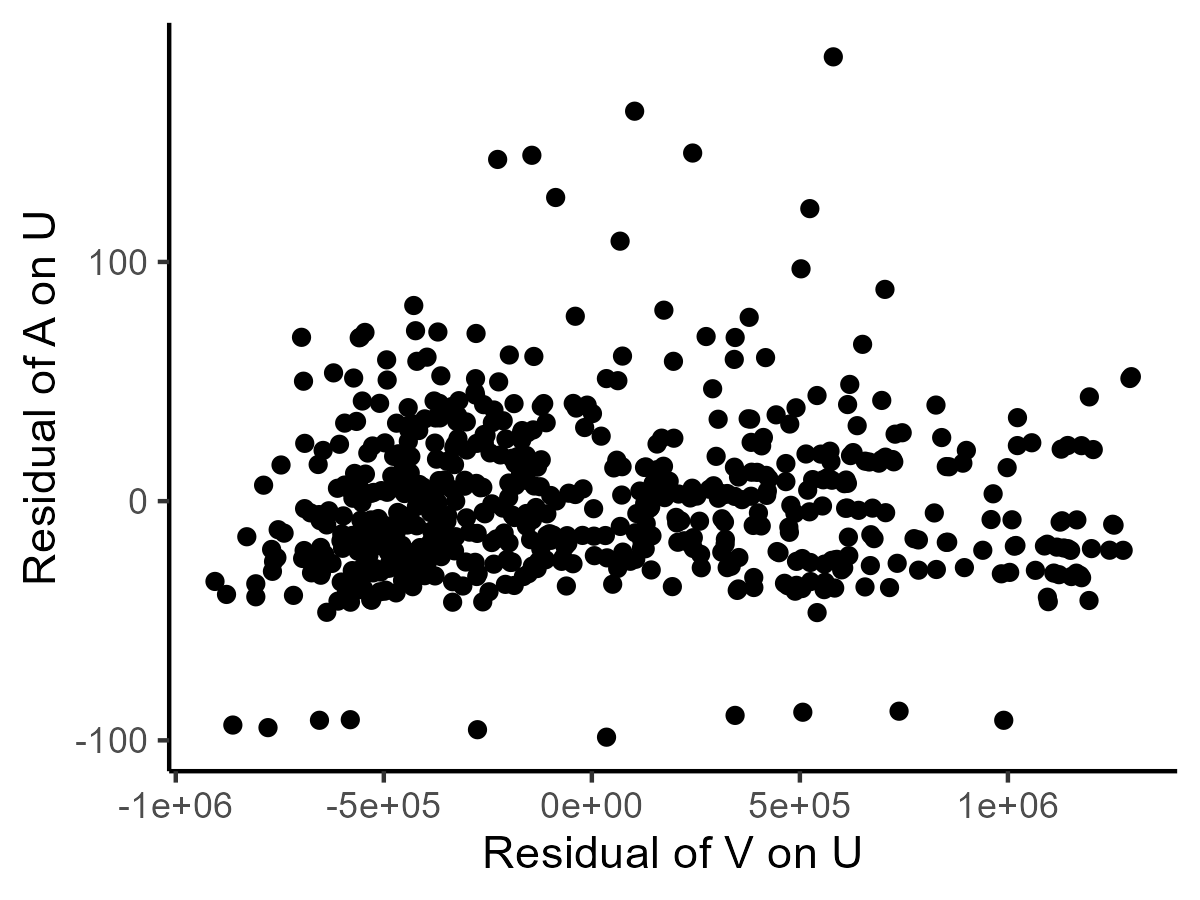
\includegraphics[width = 0.33\textwidth]
  {figuretable/residual_plot_month_aggregate.png}}
  % \subfloat[Year-level part-time and full-time]{\includegraphics[width = 0.33\textwidth]
  % {figuretable/residual_plot_year.png}}
  \subfloat[Full-time]{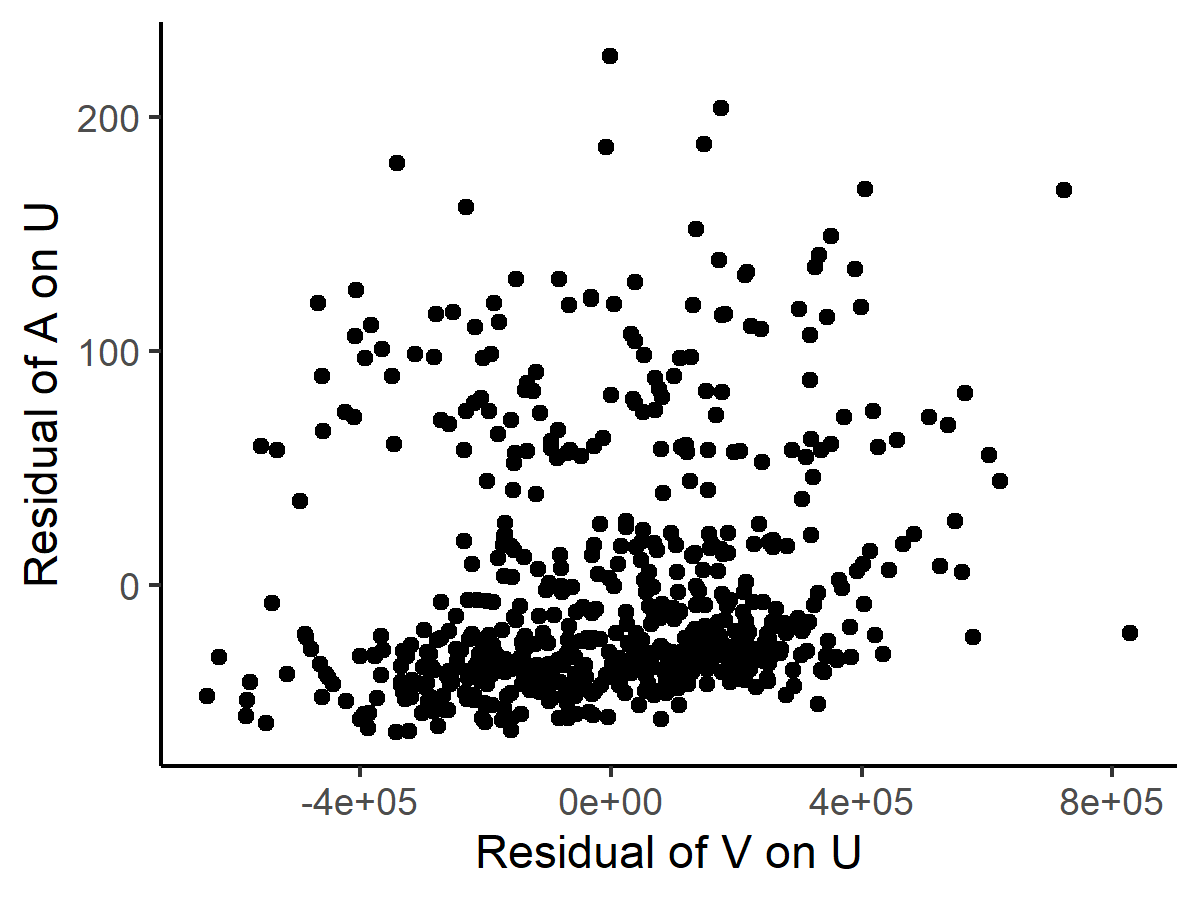
\includegraphics[width = 0.37\textwidth]
  {figuretable/residual_plot_month_full_time.png}}
  \subfloat[Part-time]{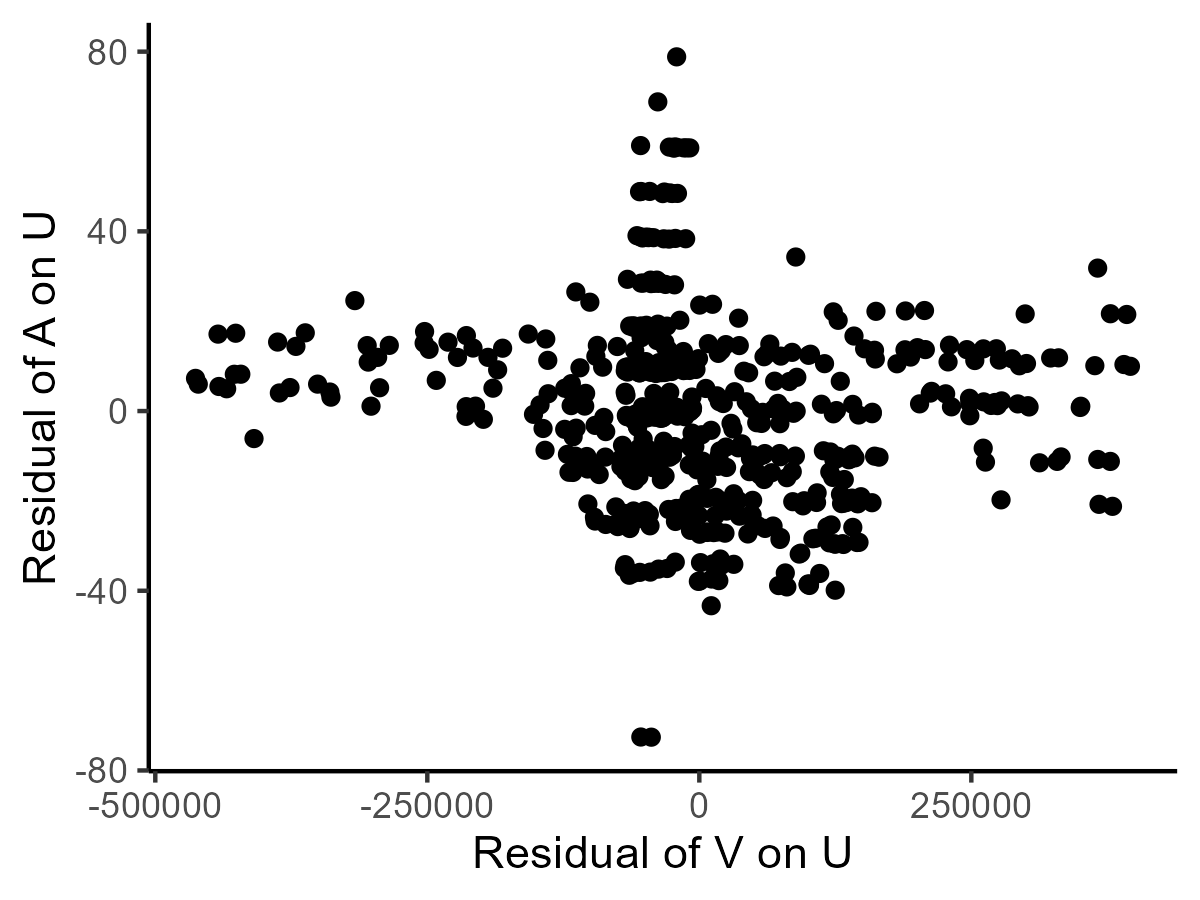
\includegraphics[width = 0.33\textwidth]
  {figuretable/residual_plot_month_part_time.png}}
  \caption{Residual plot}
  \label{fg:residual_plots} 
  \end{center}
  \footnotesize
  %Note: 
\end{figure} 


\subsection{Aggregate trends in 1972-2023}\label{sec:month_level}

Figures \ref{fg:month_part_and_full_time_results} (a)-(d) provide monthly data patterns of unemployed individuals, vacancies, labor market tightness (\(V/U\)), hires, the  ($U$,$V$) relationship, and job and worker finding rates (\(M/U\) and \(M/V\)) in aggregate labor markets. 
In summary, the numbers of unemployed individuals and vacancies increase with fluctuations, corresponding with market tightness, while the number of hires shows a noticeable decline around the late 1970s, peaks and troughs from the mid-1980s to the late 1990s, peaks around mid-2000s and 2010, and a sharp decline towards recent years.
Although the ($U$,$V$) relationship does not corresponds with Beveridge curve because these numbers are not divided by the corresponding number of labor force, the prominent rightward shifts are consistent with the previous studies \citep{elsby2015beveridge}.

Figures \ref{fg:month_part_and_full_time_results} (e) and (f) present the estimation results of the matching function along with matching efficiency and elasticities (\(\frac{d\ln M}{d\ln U}\) and \(\frac{d\ln M}{d\ln V}\)). Notably, matching efficiency (normalized to 1972) shows a declining trend with notable fluctuations, which is consistent with the downward trends of job and worker finding rates. 
In particular, the significant decline after 2015 is remarkable.
This seems due to an increase in matching opportunities outside of the government-operated platform.

The implied match elasticity with respect to unemployment is 0.5-0.9, which is comparable to previous worldwide findings such as \cite{petrongolo2001looking} (range: 0.5-0.7) and Japanese studies such as \cite{higashi2018spatial} (0.38 for 2000-2014 monthly), \cite{kawata2019} (0.48 for 2012-2017 prefecture-month-level), \cite{kano2005estimating} (0.56 for 1972-1999 prefecture-year-level), \cite{sasaki2007measuring} (about 0.6 for 1998-2007 prefecture-quarter-level), and \cite{kambayashi2006vacancy} (about 0.8 for 1996-2001 prefecture-month-level). However, I discuss the need for careful interpretation of the estimates due to scale normalization of matching efficiency in Section \ref{sec:month_level}.\footnote{For reference, \cite{petrongolo2001looking} summarize early aggregate studies in many countries based on a Cobb-Douglas matching function with the flow of hires on the left-hand side and the stock of unemployment and job vacancies on the right-hand side. In short, match elasticity with respect to unemployment is in the range of 0.5–0.7.}
Also, the implied match elasticity with respect to vacancies is 0.1-0.4, which is comparable to \cite{lange2020beyond} (range: 0.3-0.5) and Japanese studies such as \cite{higashi2018spatial} (0.24 for 2000-2014 monthly), \cite{kawata2019} (0.52 for 2012-2017 prefecture-month-level), \cite{kano2005estimating} (0.3 for 1972-1999 prefecture-year-level), \cite{sasaki2007measuring} (about 0.2 for 1998-2007 prefecture-quarter-level), and \cite{kambayashi2006vacancy} (about 0.3 for 1996-2001 prefecture-month-level).

Figures \ref{fg:month_part_and_full_time_results} (g) and (h) illustrate some correlation patterns between matching efficiency and market structure variables such as labor market tightness, worker finding rate, and job finding rate. Consistent with \cite{lange2020beyond}, these highlight positive correlations between efficiency and market structure, such as tightness, which induce a positive bias in the estimates of the vacancy elasticity whenever unobserved matching efficacy is not controlled for, as is the case in traditional estimators.


\begin{figure}[!ht]
  \begin{center}
  \subfloat[Unemployed ($U$), Vacancy ($V$), and Tightness ($\frac{V}{U}$)]{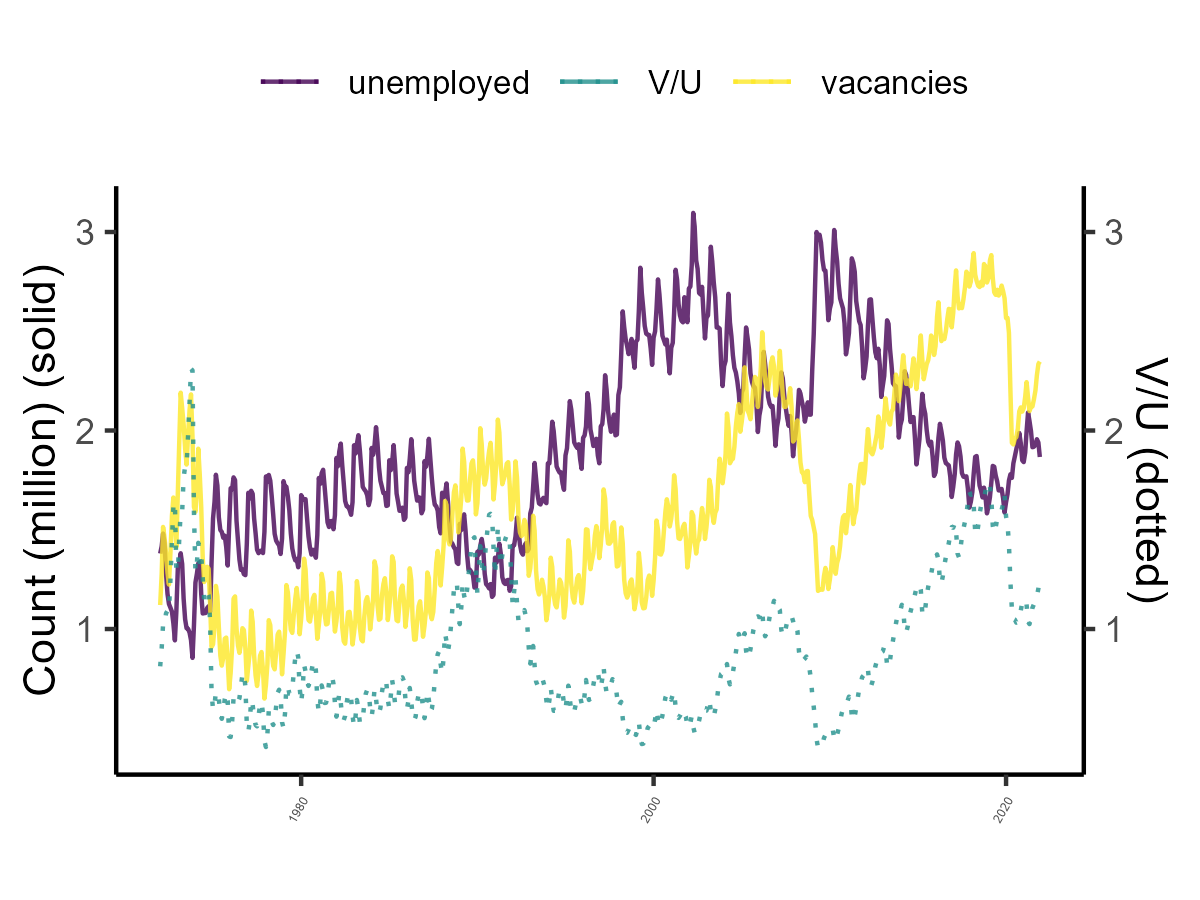
\includegraphics[width = 0.37\textwidth]
  {figuretable/unemployed_vacancy_month_aggregate.png}}
  \subfloat[Hire ($H$)]{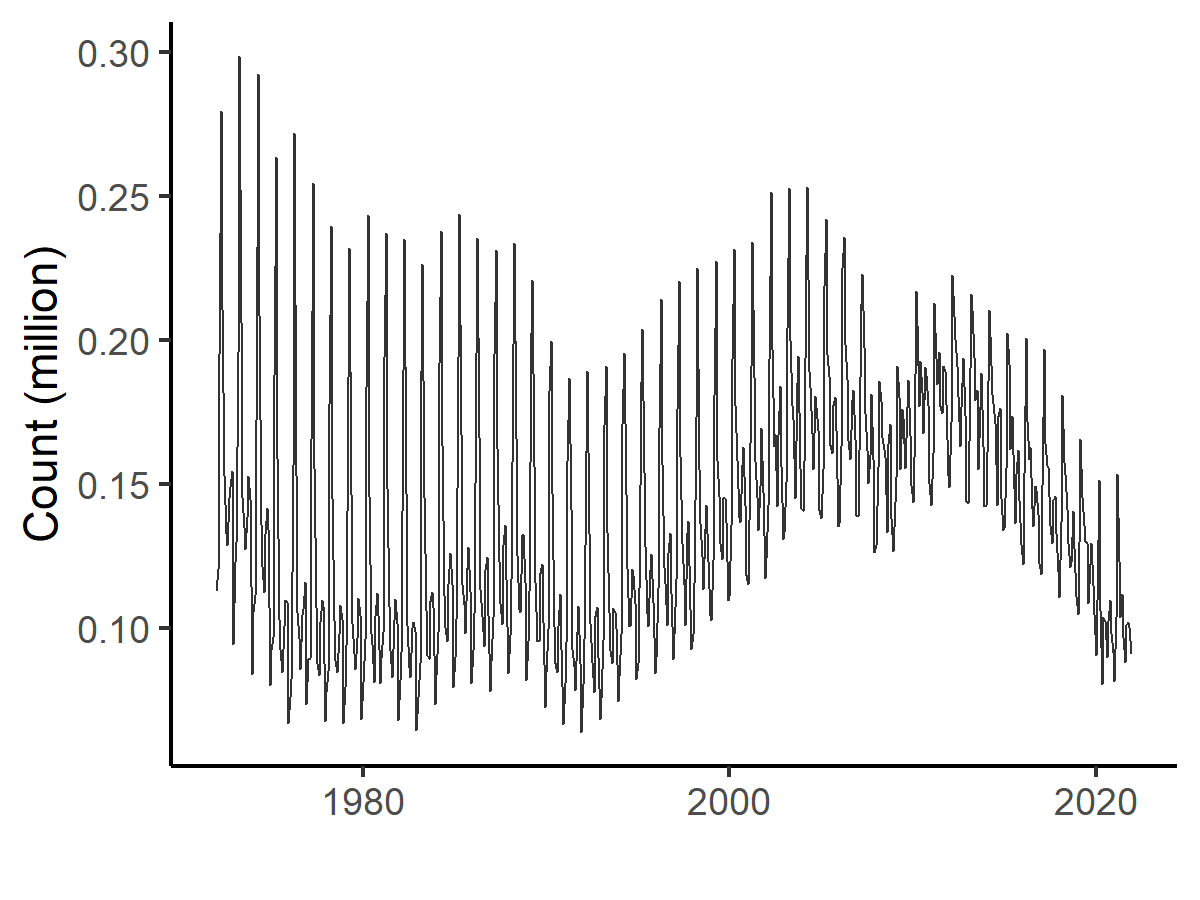
\includegraphics[width = 0.37\textwidth]
  {figuretable/hire_month_aggregate.png}}\\
  \subfloat[ ($U$,$V$) relationship]{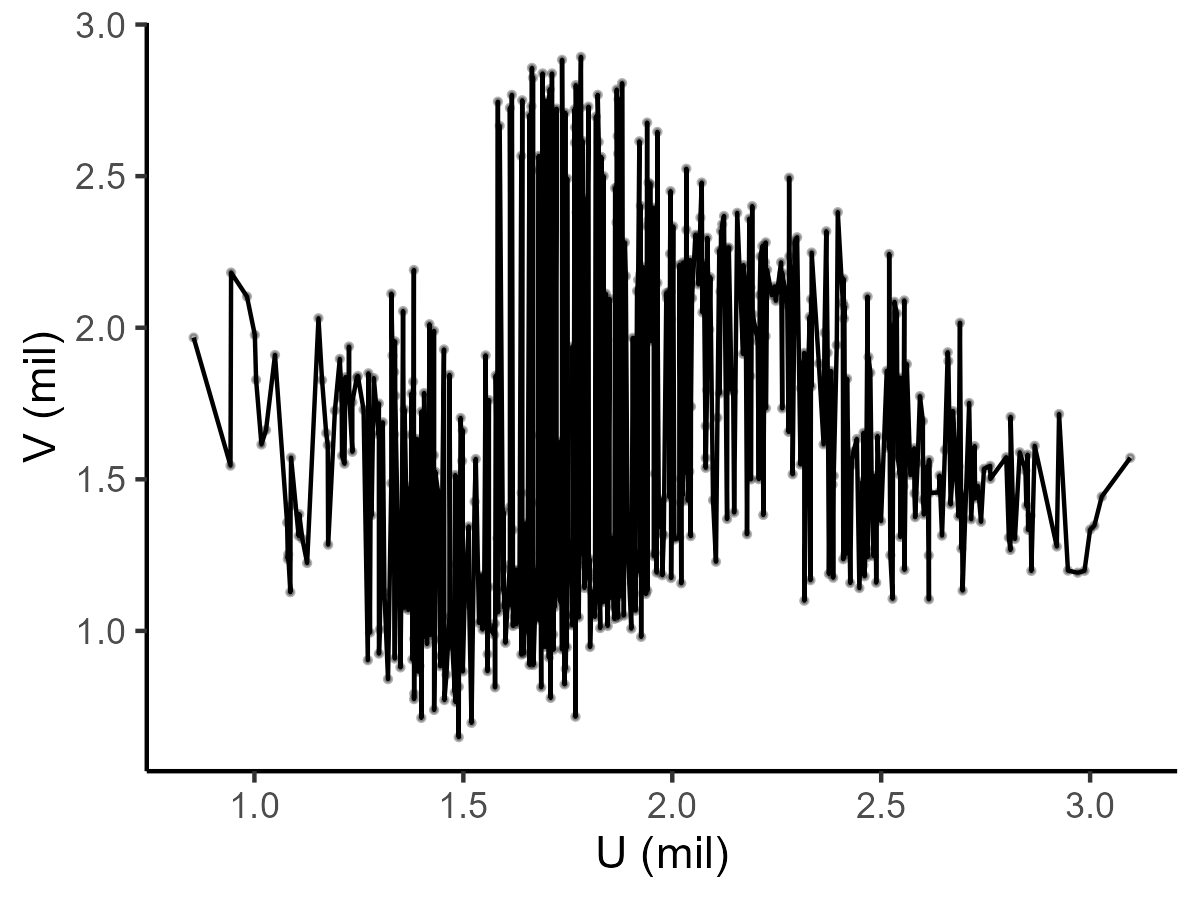
\includegraphics[width = 0.37\textwidth]
  {figuretable/unemployed_vacancies_berveridge_month_aggregate.png}}
  \subfloat[Job Worker finding rate ($\frac{M}{U}$,$\frac{M}{V}$)]{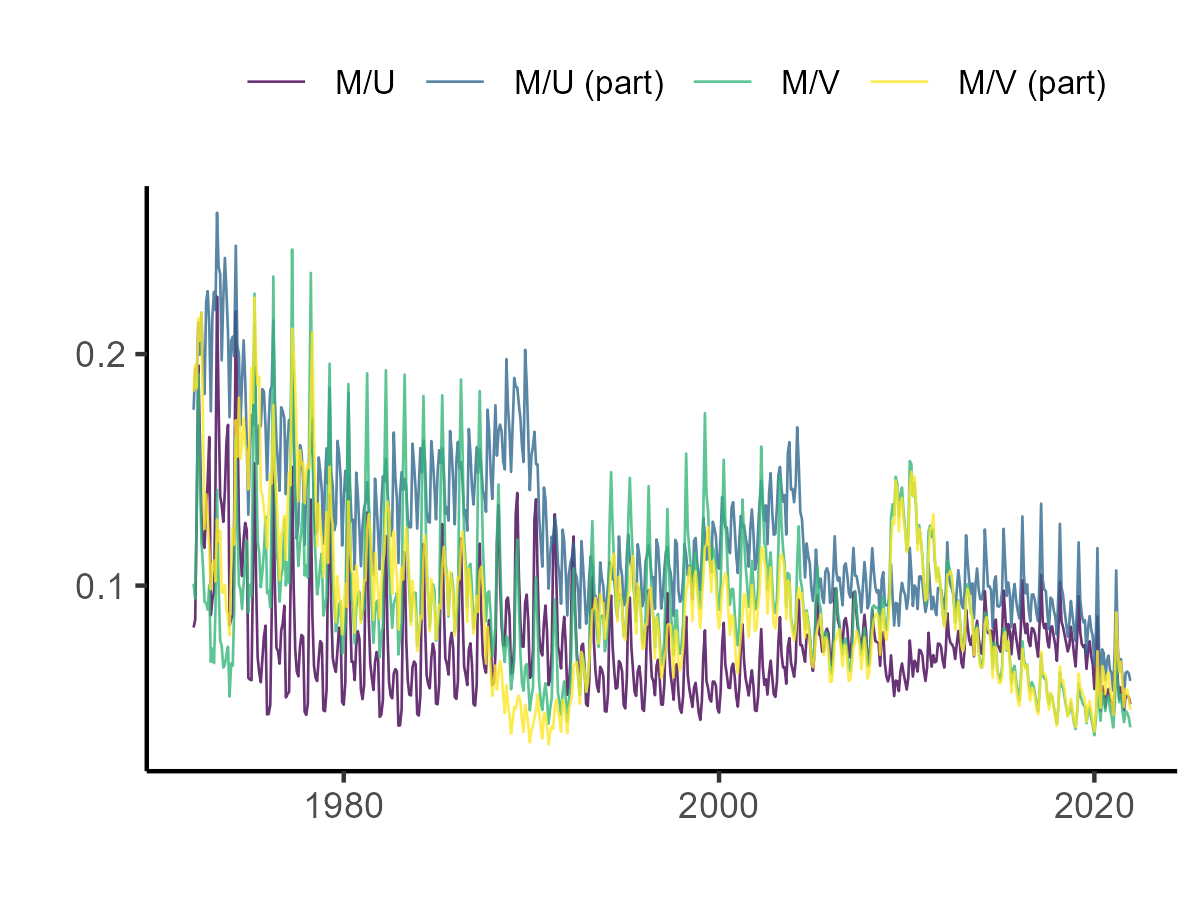
\includegraphics[width = 0.37\textwidth]
  {figuretable/job_finding_rate_worker_finding_rate_month_aggregate.png}}
  \\
  \subfloat[Matching Efficiency ($A$)]{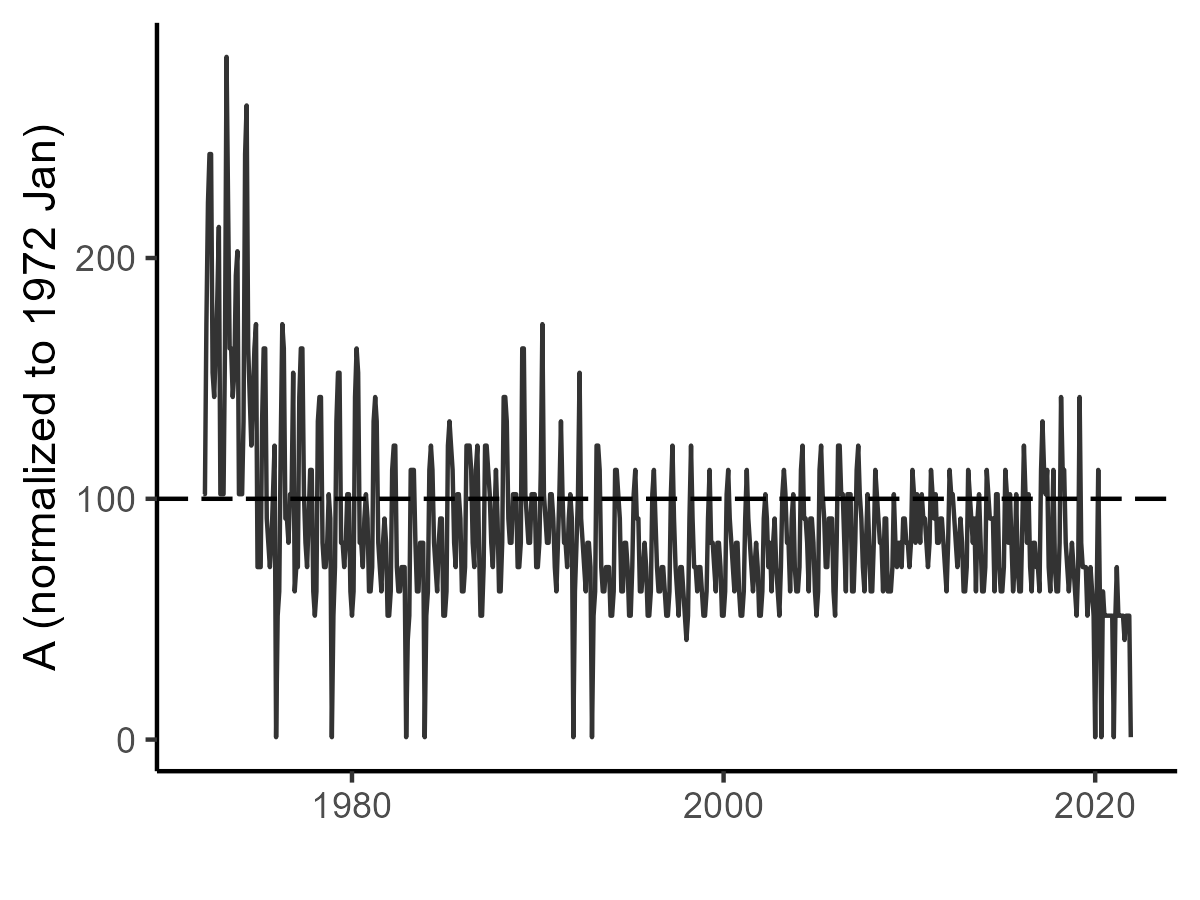
\includegraphics[width = 0.37\textwidth]
  {figuretable/matching_efficiency_month_aggregate.png}}
  \subfloat[Matching Elasticity ($\frac{d\ln M}{d \ln AU}$, $\frac{d\ln M}{d\ln V}$)]{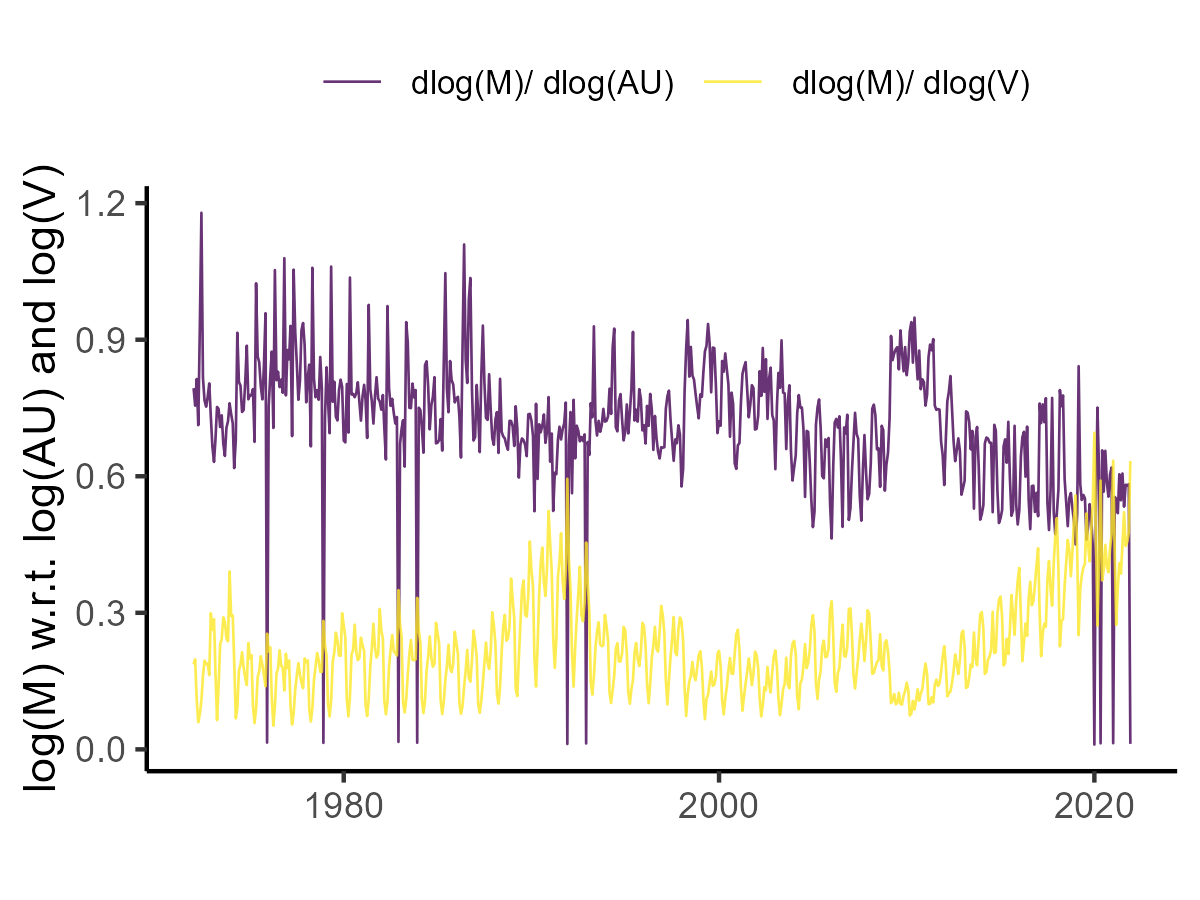
\includegraphics[width = 0.37\textwidth]
  {figuretable/elasticity_month_aggregate.png}}\\
  \subfloat[Efficiency ($A$) and Tightness ($\ln\frac{V}{U}$)]{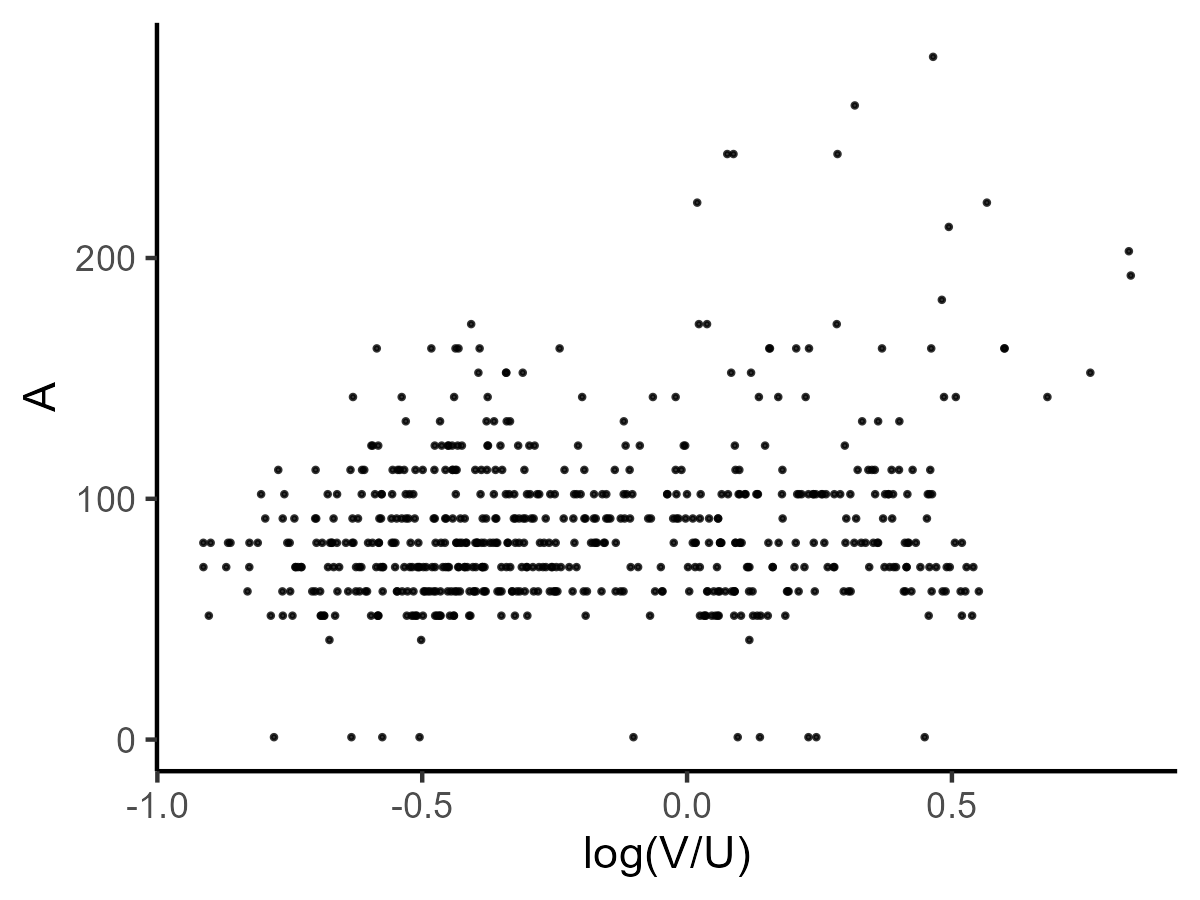
\includegraphics[width = 0.37\textwidth]
  {figuretable/efficiency_tightness_plot_month_aggregate.png}}
  \subfloat[Efficiency ($A$) and ($\ln\frac{M}{U}$, $\ln\frac{M}{V}$)]{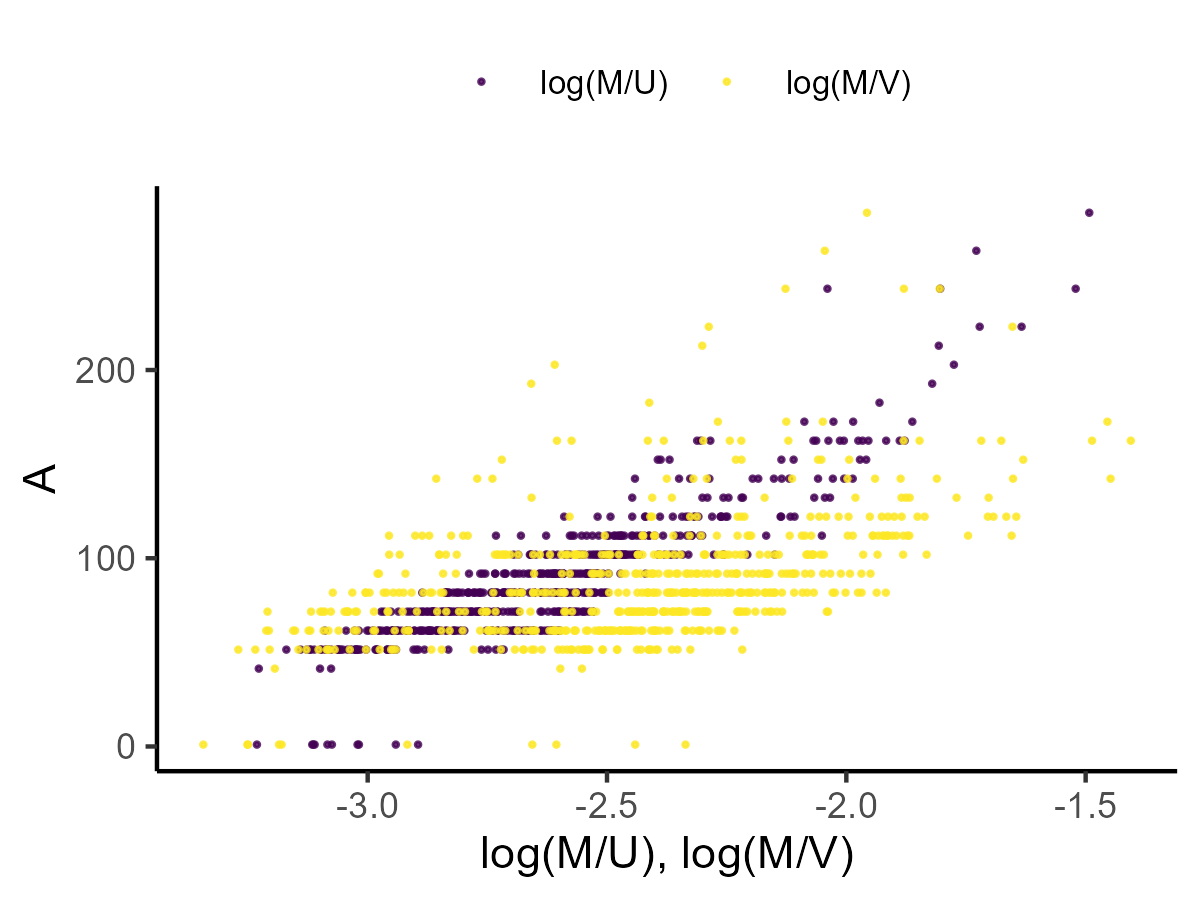
\includegraphics[width = 0.37\textwidth]
  {figuretable/job_finding_rate_efficiency_plot_month_aggregate.png}}
  \caption{Month-level aggregate results 1972-2024}
  \label{fg:month_part_and_full_time_results} 
  \end{center}
  \footnotesize
  %Note: 
\end{figure} 




\subsection{Decomposition of part-time and full time trends in 1972-2023}
Next we decompose the aggregate trends into full-time and part-time labor markets' trends.
Figure \ref{fg:month_full_time_part_time_results} provide full-time and part-time labor markets' trends corresponding Figures \ref{fg:month_part_and_full_time_results} (a)-(f).

Figure \ref{fg:month_full_time_part_time_correlation_results} corresponds with Figures \ref{fg:month_part_and_full_time_results} (g)-(h).



\begin{figure}[!ht]
  \begin{center}
  \subfloat[Unemployed ($U$), Vacancy ($V$), and Tightness ($\frac{V}{U}$)]{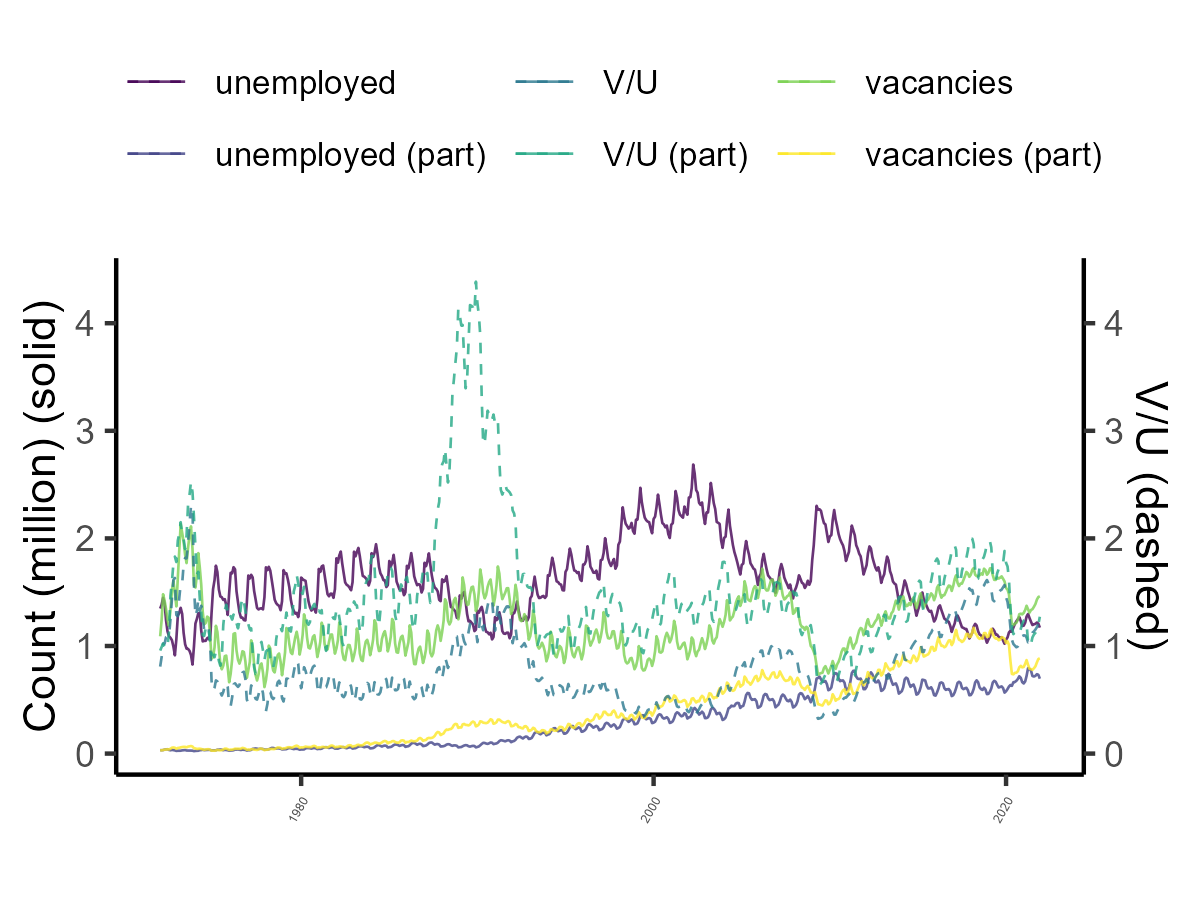
\includegraphics[width = 0.37\textwidth]
  {figuretable/unemployed_vacancy_month_full_time_part_time.png}}
  \subfloat[Hire ($H$)]{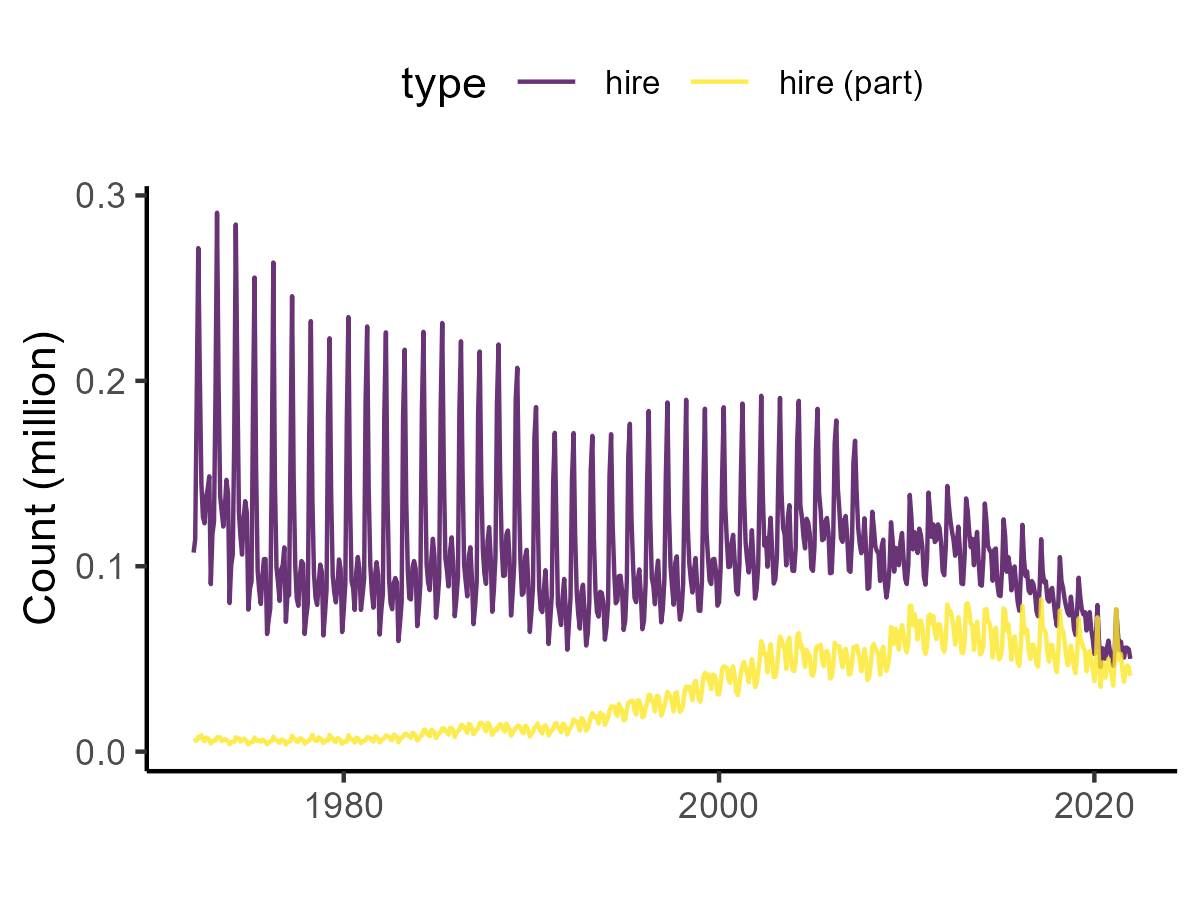
\includegraphics[width = 0.37\textwidth]
  {figuretable/hire_month_full_time_part_time.png}}\\
  \subfloat[ ($U$,$V$) relationship]{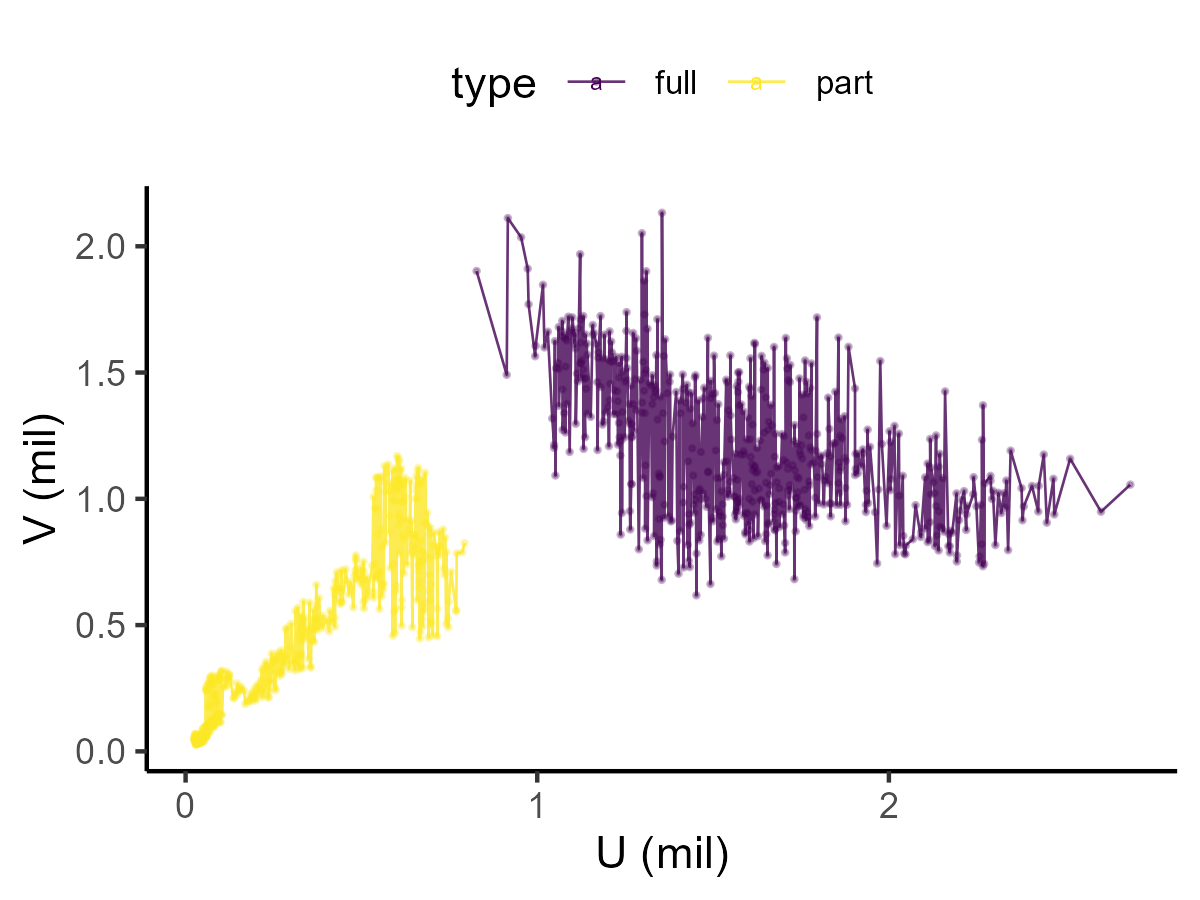
\includegraphics[width = 0.37\textwidth]
  {figuretable/unemployed_vacancies_berveridge_month_full_time_part_time.png}}
  \subfloat[Job Worker finding rate ($\frac{M}{U}$,$\frac{M}{V}$)]{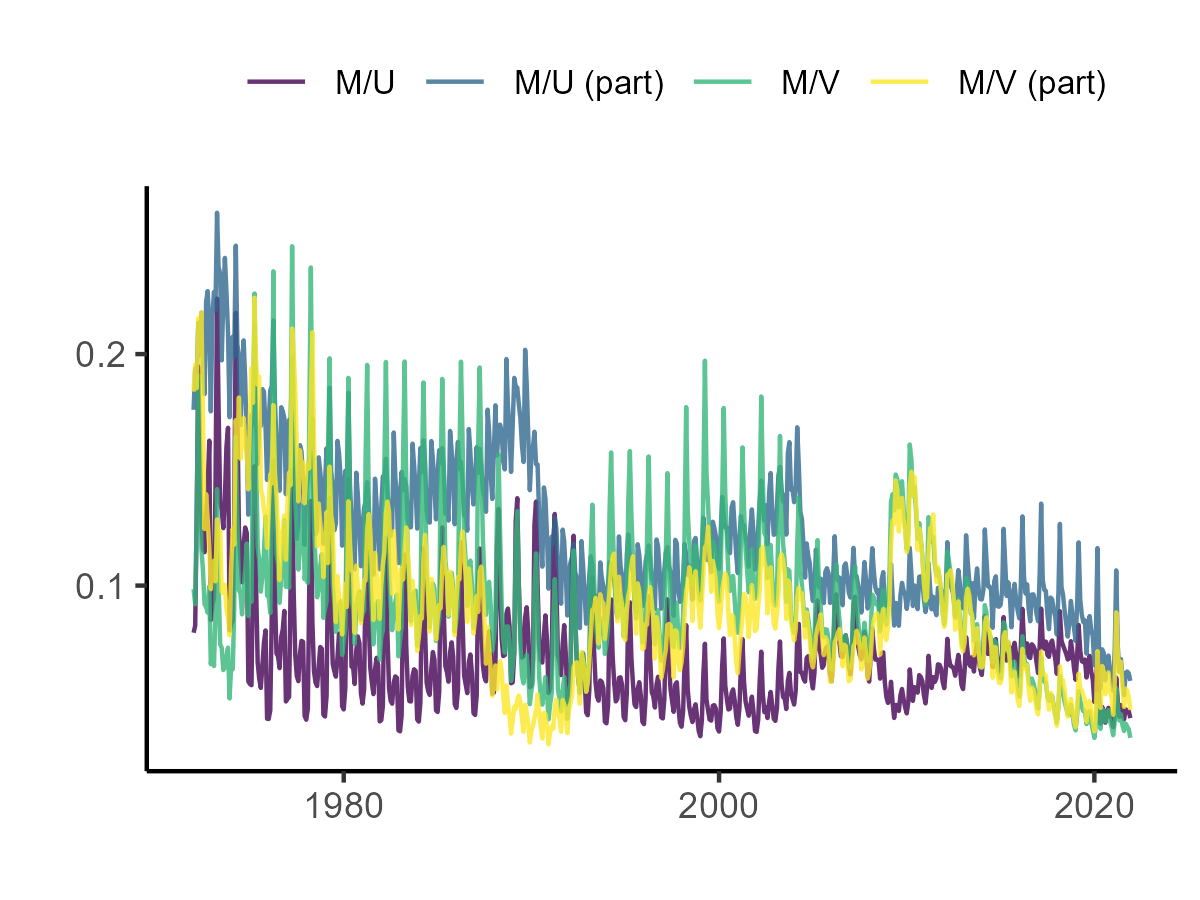
\includegraphics[width = 0.37\textwidth]
  {figuretable/job_finding_rate_worker_finding_rate_month_full_time_part_time.png}}
  \\
  \subfloat[Matching Efficiency ($A$)]{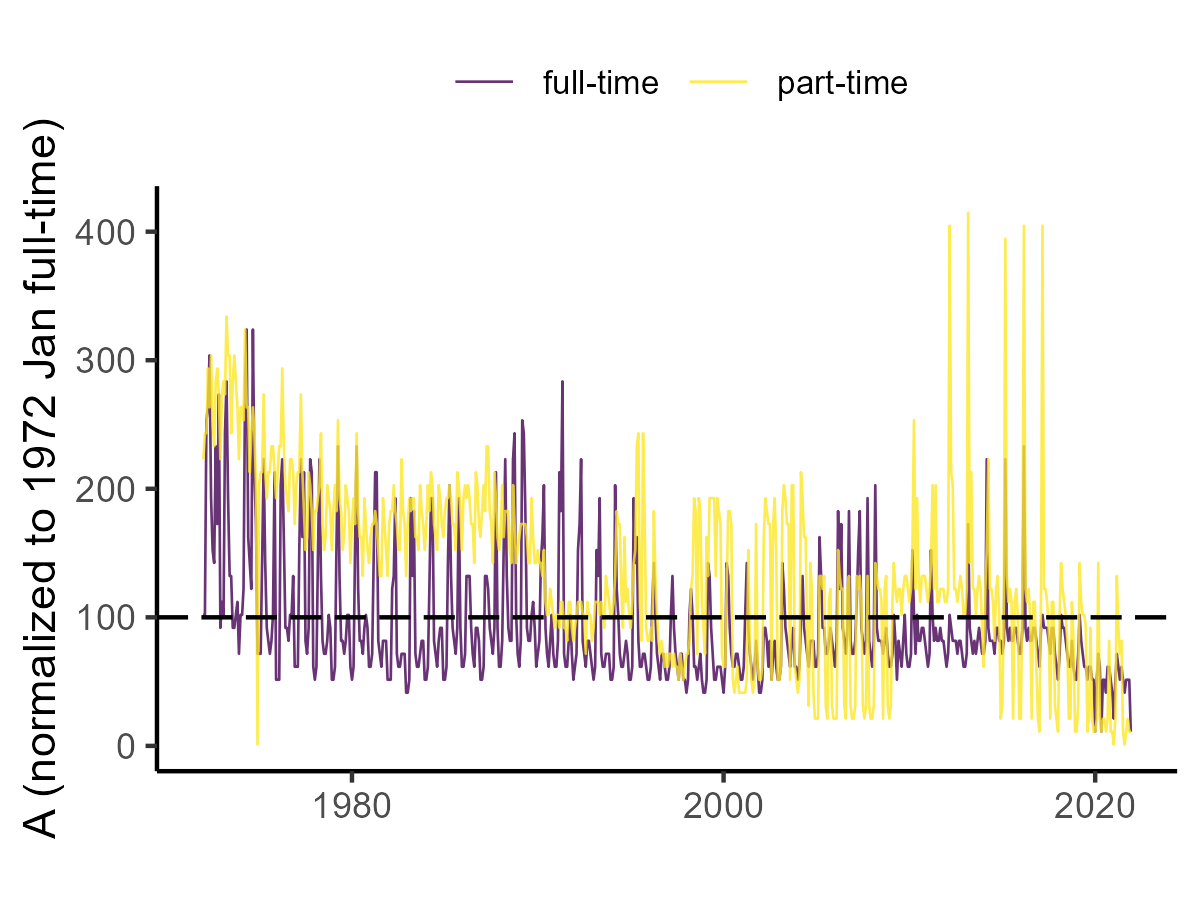
\includegraphics[width = 0.37\textwidth]
  {figuretable/matching_efficiency_month_full_time_part_time.png}}
  \subfloat[Matching Elasticity ($\frac{d\ln M}{d \ln AU}$, $\frac{d\ln M}{d\ln V}$)]{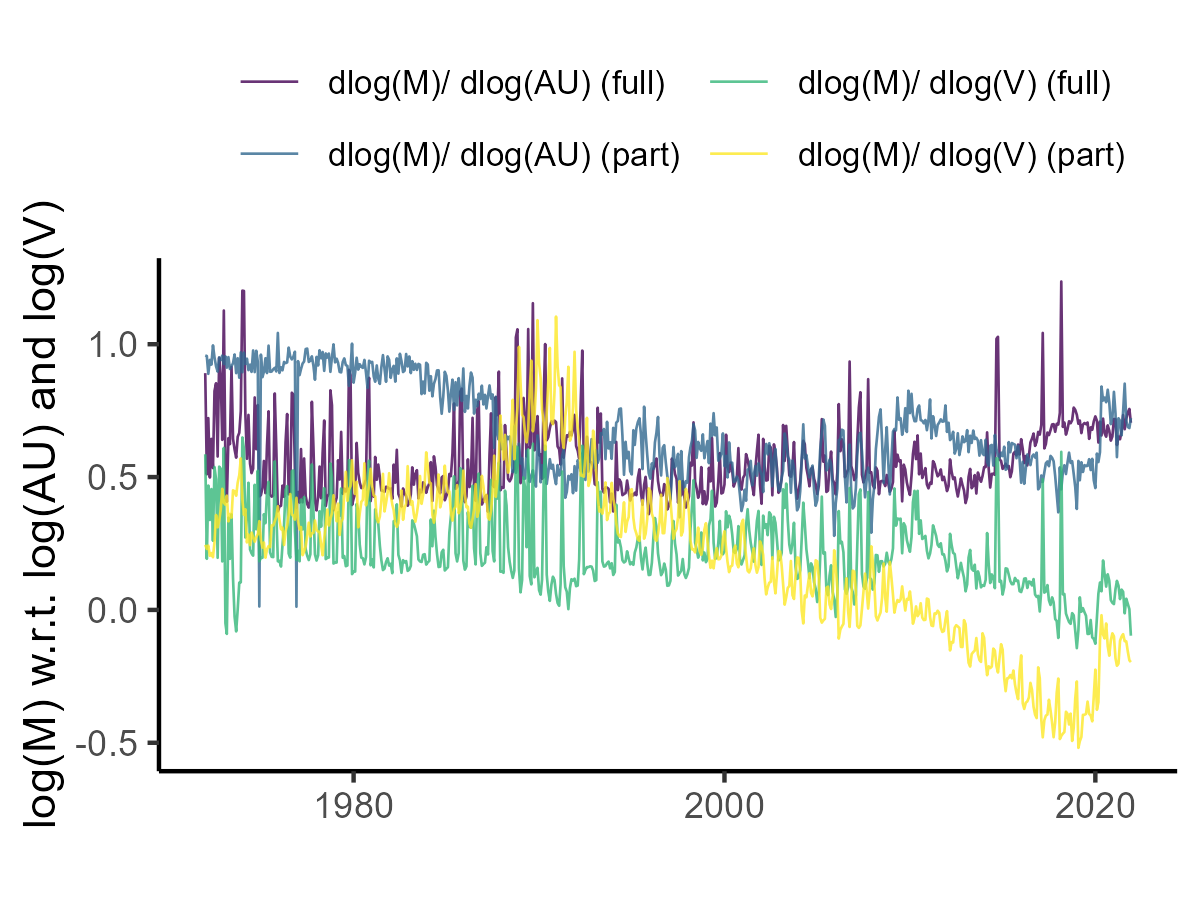
\includegraphics[width = 0.37\textwidth]
  {figuretable/elasticity_month_full_time_part_time.png}}
  % \\
  % \subfloat[Efficiency ($A$) and Tightness ($\ln\frac{V}{U}$)]{\includegraphics[width = 0.37\textwidth]
  % {figuretable/efficiency_tightness_plot_month_full_time.png}}
  % \subfloat[Efficiency ($A$) and ($\ln\frac{M}{U}$, $\ln\frac{M}{V}$)]{\includegraphics[width = 0.37\textwidth]
  % {figuretable/job_finding_rate_efficiency_plot_month_full_time.png}}
  \caption{Month-level full-time and part-time results 1972-2024}
  \label{fg:month_full_time_part_time_results} 
  \end{center}
  \footnotesize
  %Note: 
\end{figure} 


\begin{figure}[!ht]
  \begin{center}
  \subfloat[Efficiency ($A$) and Tightness ($\ln\frac{V}{U}$), Part-time (left) and Full-time (right)]{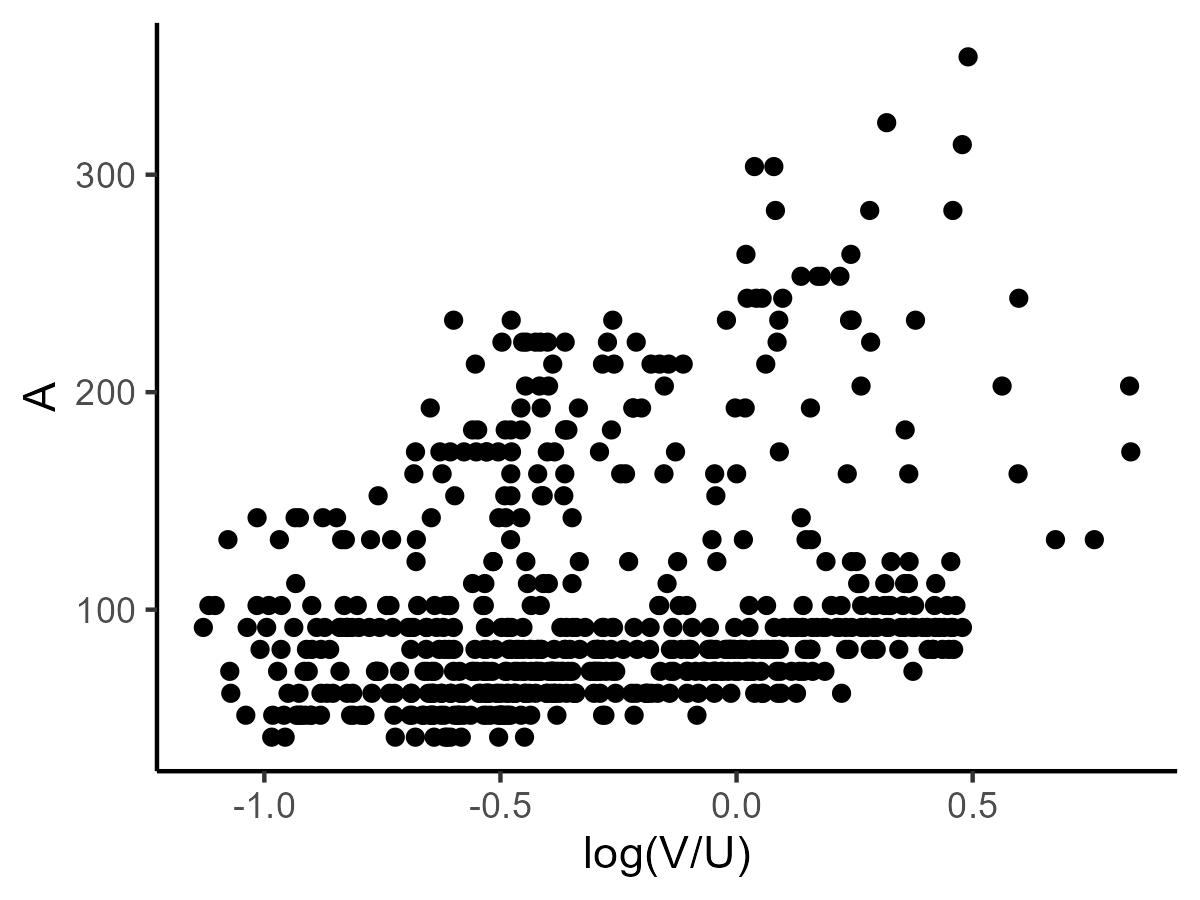
\includegraphics[width = 0.37\textwidth]
  {figuretable/efficiency_tightness_plot_month_full_time.png}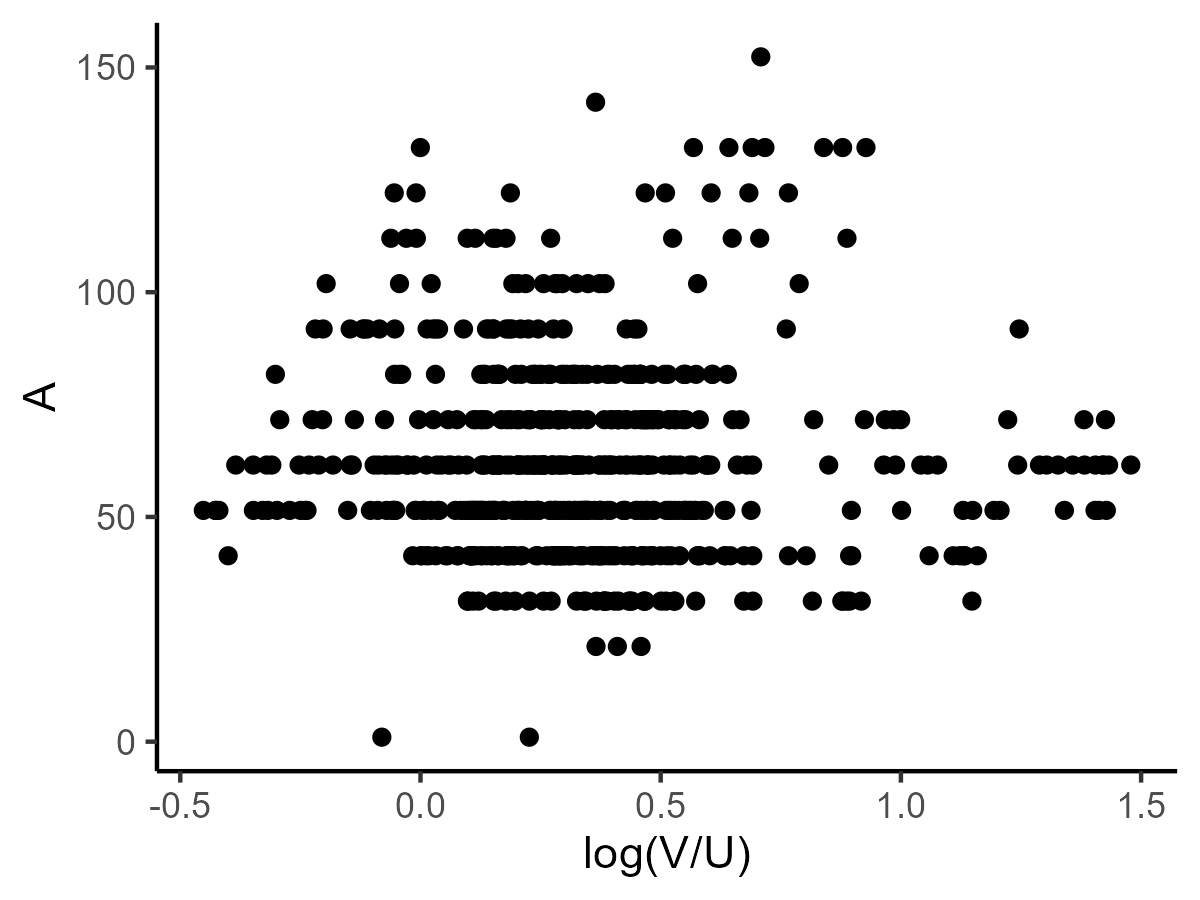
\includegraphics[width = 0.37\textwidth]
  {figuretable/efficiency_tightness_plot_month_part_time.png}}\\
  \subfloat[Efficiency ($A$) and ($\ln\frac{M}{U}$, $\ln\frac{M}{V}$), Part-time (left) and Full-time (right)]{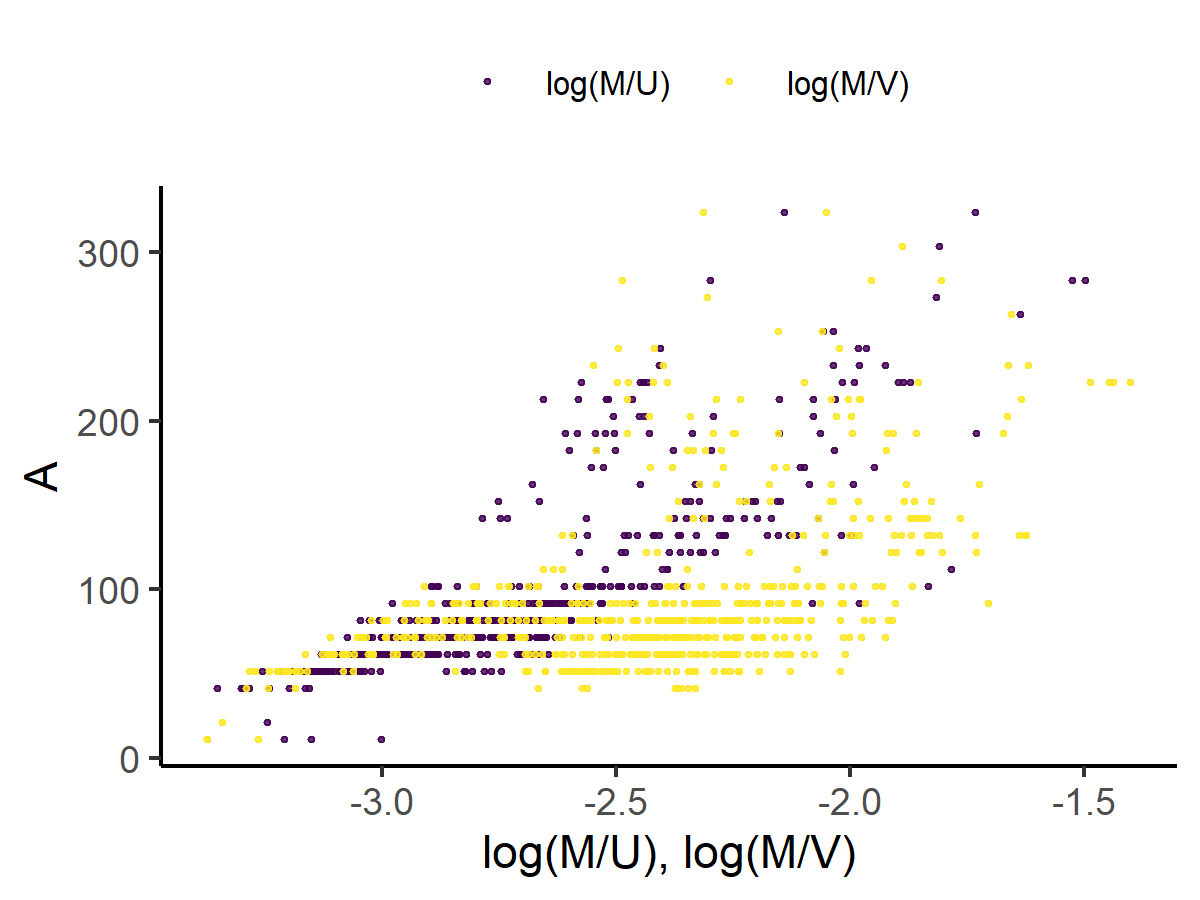
\includegraphics[width = 0.37\textwidth]
  {figuretable/job_finding_rate_efficiency_plot_month_full_time.png}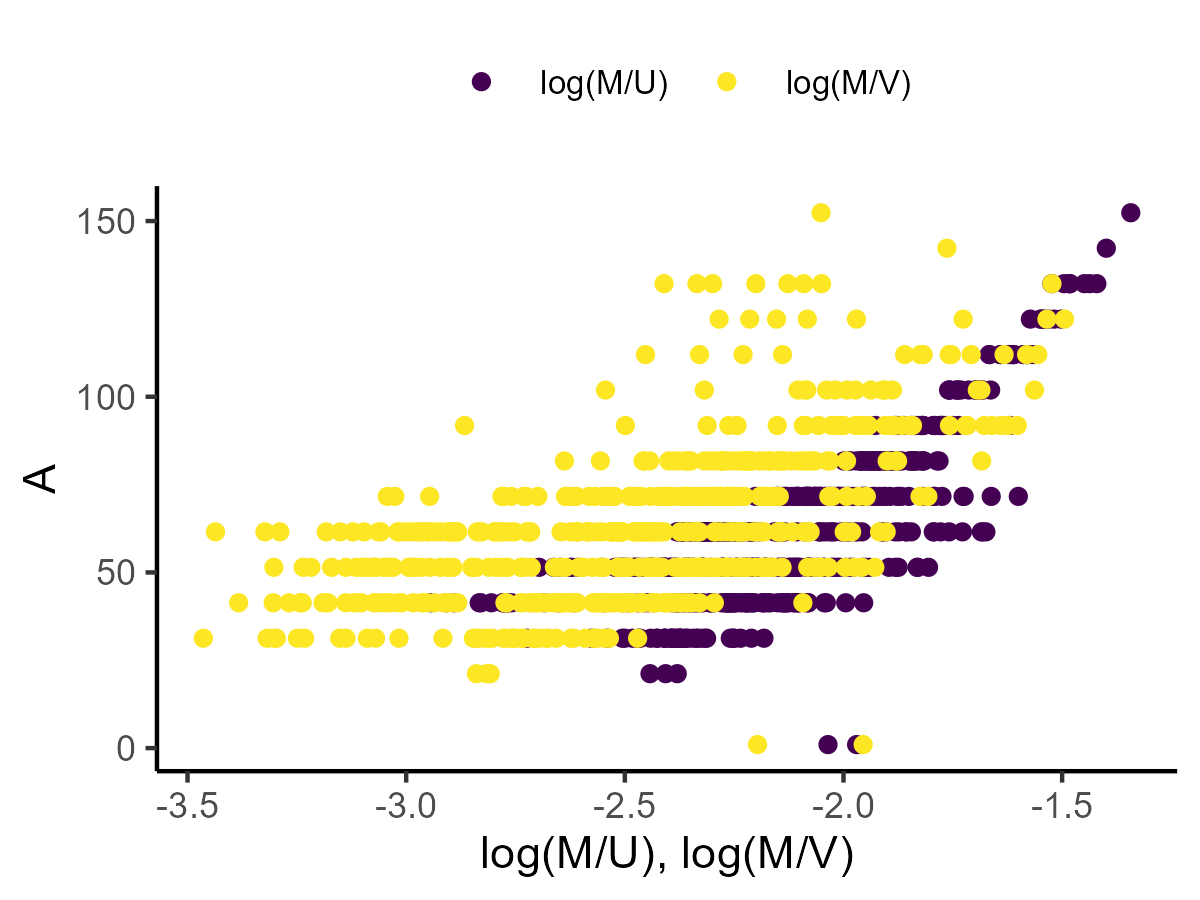
\includegraphics[width = 0.37\textwidth]
  {figuretable/job_finding_rate_efficiency_plot_month_part_time.png}}
  \caption{Month-level full-time and part-time results 1972-2024}
  \label{fg:month_full_time_part_time_correlation_results} 
  \end{center}
  \footnotesize
  %Note: 
\end{figure} 





\subsection{Occupation category and prefecture level results in 2012-2024}


\begin{itemize}
    \item \textcolor{blue}{[TBA] Data collection of prefecture-level and category-level data (RA)}
    \item \textcolor{blue}{[TBA] Check the previous Japanese studies meticulously again and construct the list of elasticity results. (RA)}
    \item \textcolor{blue}{[TBA] Lasso for deriving elasticities like \cite{lange2020beyond}? (RA)}
    \item \textcolor{blue}{[TBA] Labor force $L$ data for plotting Beveridge Curve divided by $L$ for comparison of \cite{elsby2015beveridge} (RA)}
    \item Geographical Mismatch
\end{itemize}



\section{Conclusion}

I investigate how matching efficiency in the labor market via Public Employment Security Offices in Japan for unemployed workers changed during the period 1972-2024. By applying a novel nonparametric identification approach proposed by \cite{lange2020beyond} to both annual and monthly data, I find that matching efficiency (normalized to 1972) exhibits a declining trend with notable fluctuations, consistent with the downward trends in job and worker finding rates. \textcolor{blue}{[TBA] Geographical mismatch results.} Finally, I highlight that comparing matching elasticity with respect to the number of unemployed workers across different datasets is challenging due to differences in scale normalization.



% \paragraph{Acknowledgments}
% I thank Fuhito Kojima, Kosuke Uetake, Akira Matsushita, Kazuhiro Teramoto, Ryo Kambayashi, Daiji Kawaguchi, Keisuke Kawata for their valuable advice. \textcolor{blue}{This research did not receive any specific grant from funding agencies in the public, commercial, or not-for-profit sectors.[KAKENHI number]}



\bibliographystyle{ecca}
\bibliography{matching_function}

\newpage

\appendix
\section{Additional results}\label{sec:year_data}
\subsection{Year-level trends in 1966-2023}

\begin{figure}[!ht]
  \begin{center}
 \subfloat[Unemployed ($U$), Vacancy ($V$), and Tightness ($\frac{V}{U}$)]{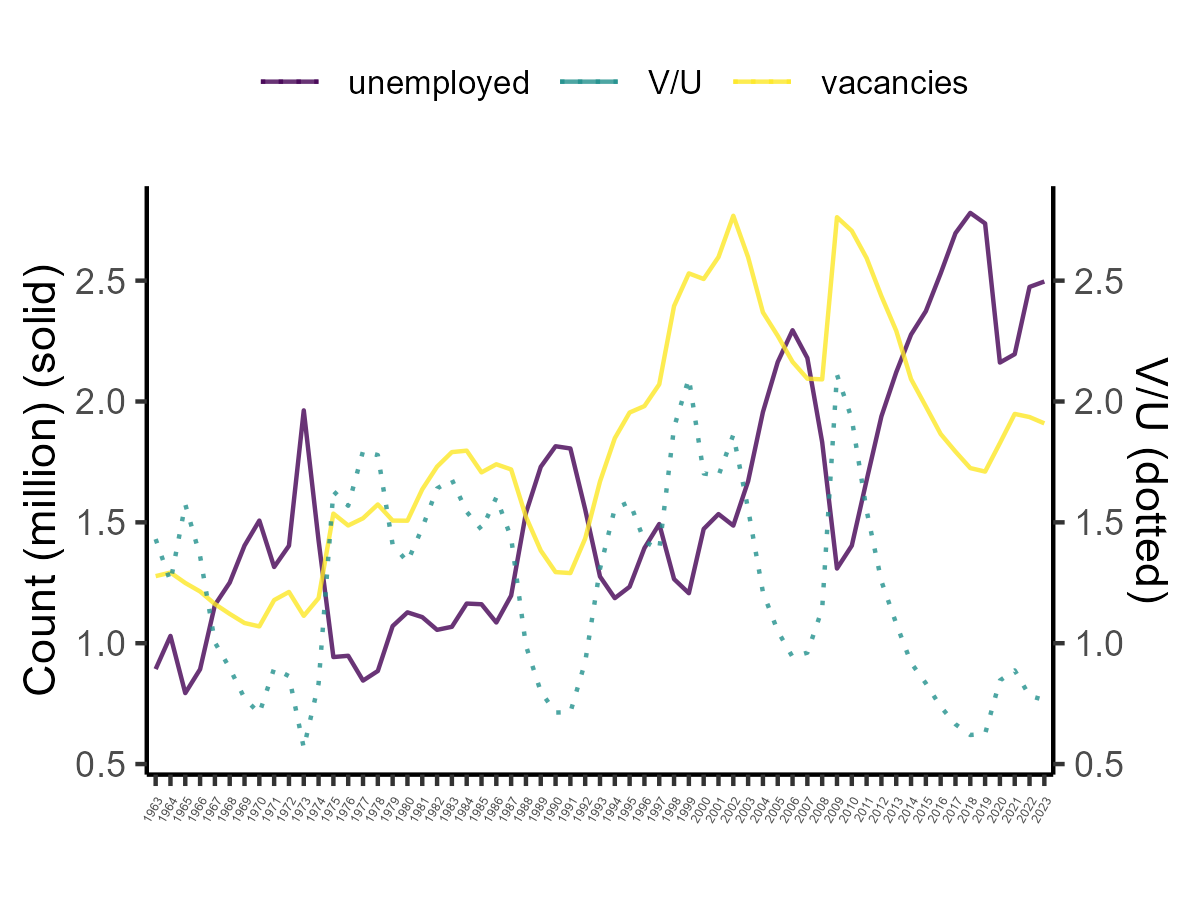
\includegraphics[width = 0.37\textwidth]
  {figuretable/unemployed_vacancy_year.png}}
  \subfloat[Hire ($H$)]{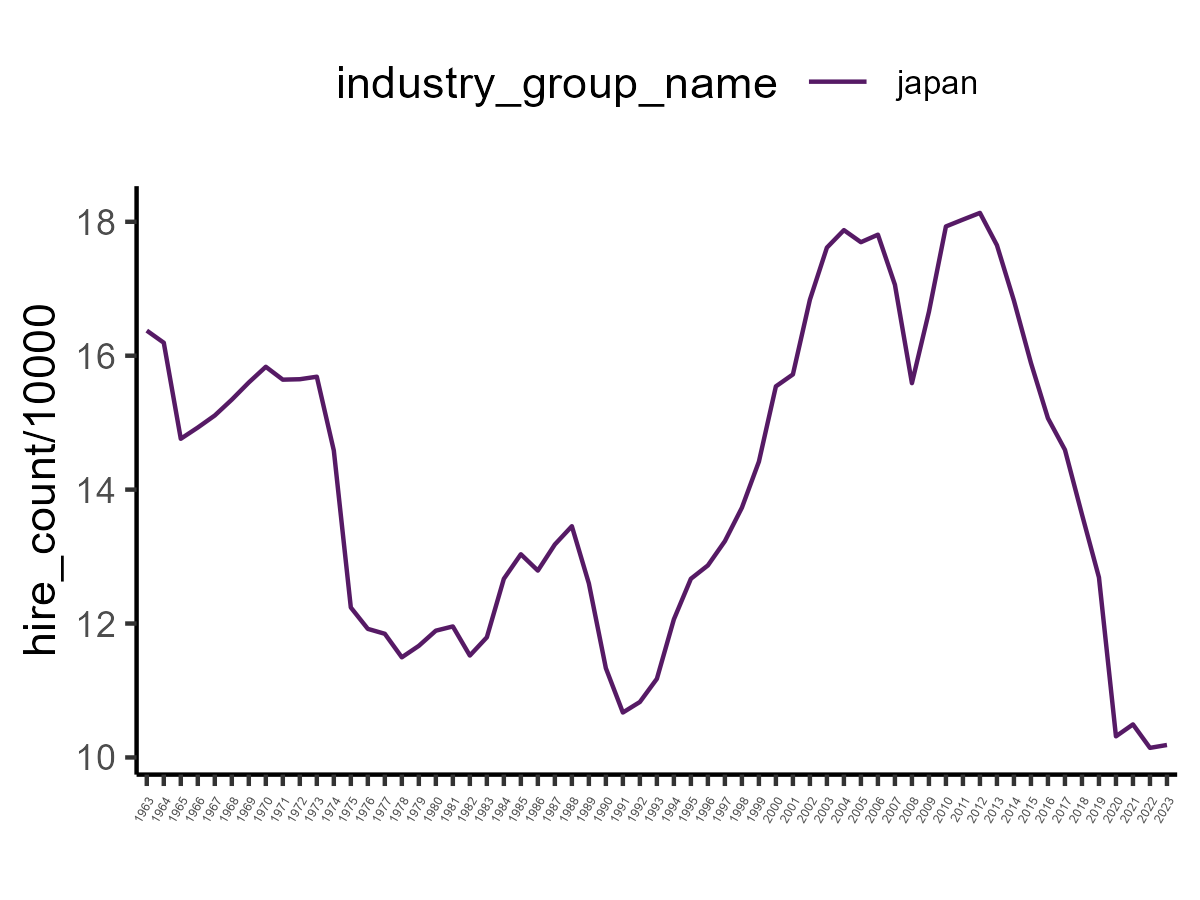
\includegraphics[width = 0.37\textwidth]
  {figuretable/hire_year.png}}\\
  \subfloat[ ($U$,$V$) relationship]{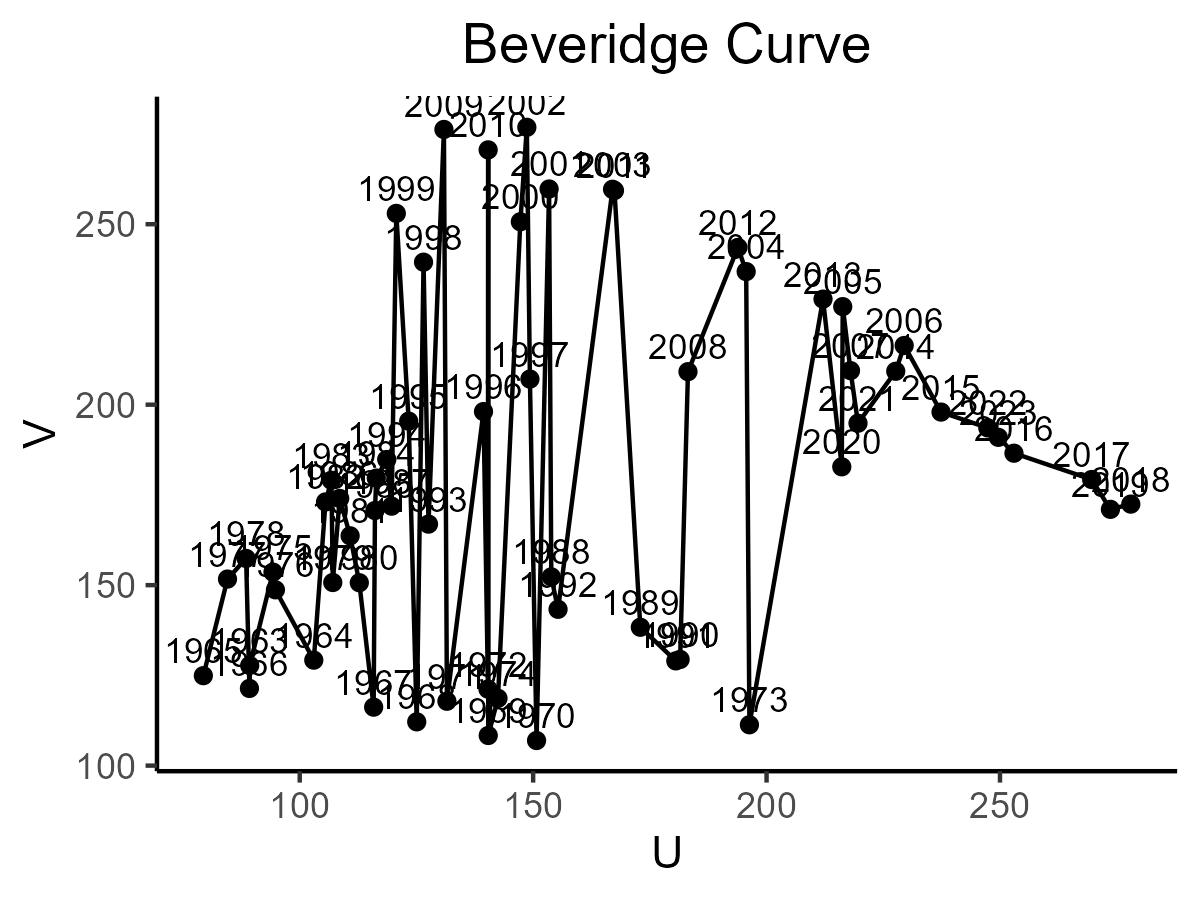
\includegraphics[width = 0.37\textwidth]
  {figuretable/unemployed_vacancies_berveridge_year.png}}
  \subfloat[Job Worker finding rate ($\frac{M}{U}$, $\frac{M}{V}$)]{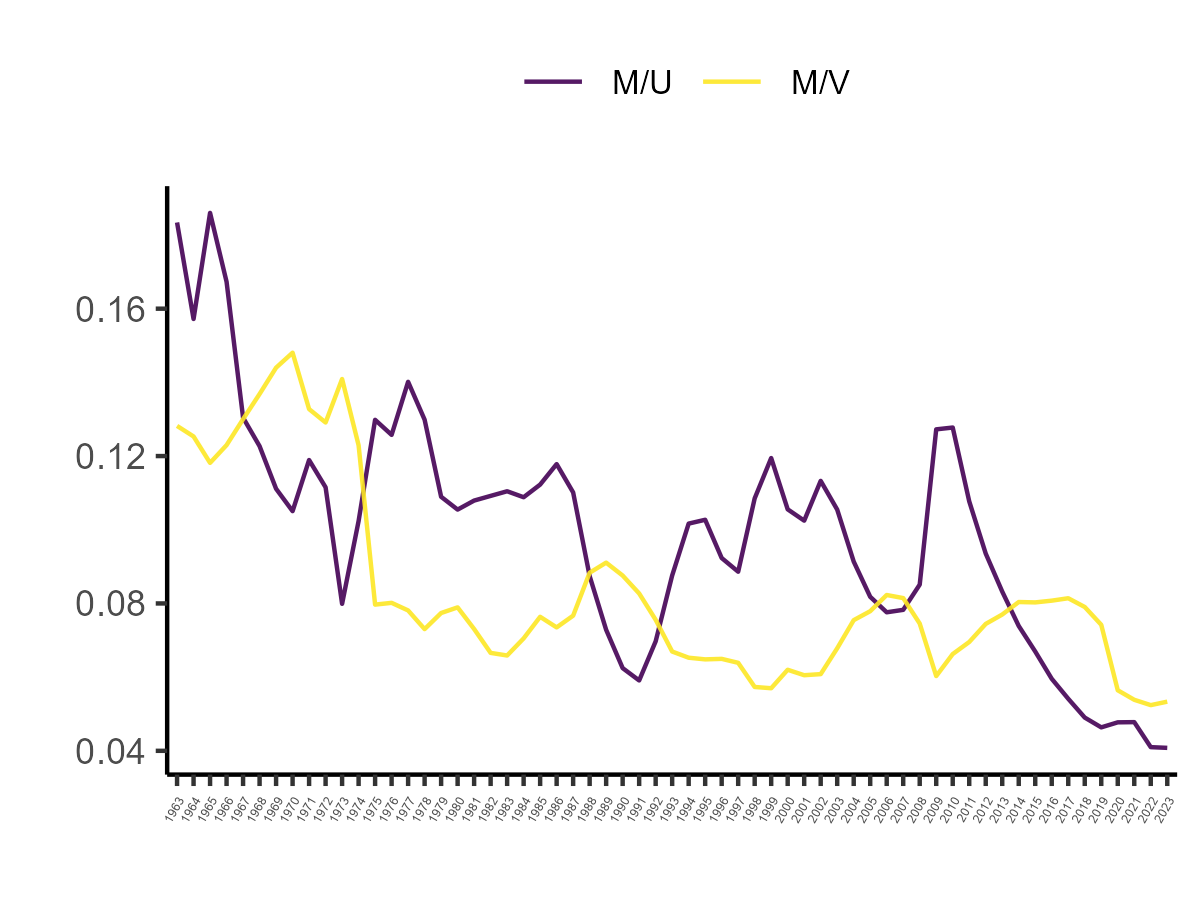
\includegraphics[width = 0.37\textwidth]
  {figuretable/job_finding_rate_worker_finding_rate_year.png}}
  \\
  \subfloat[Matching Efficiency ($A$)]{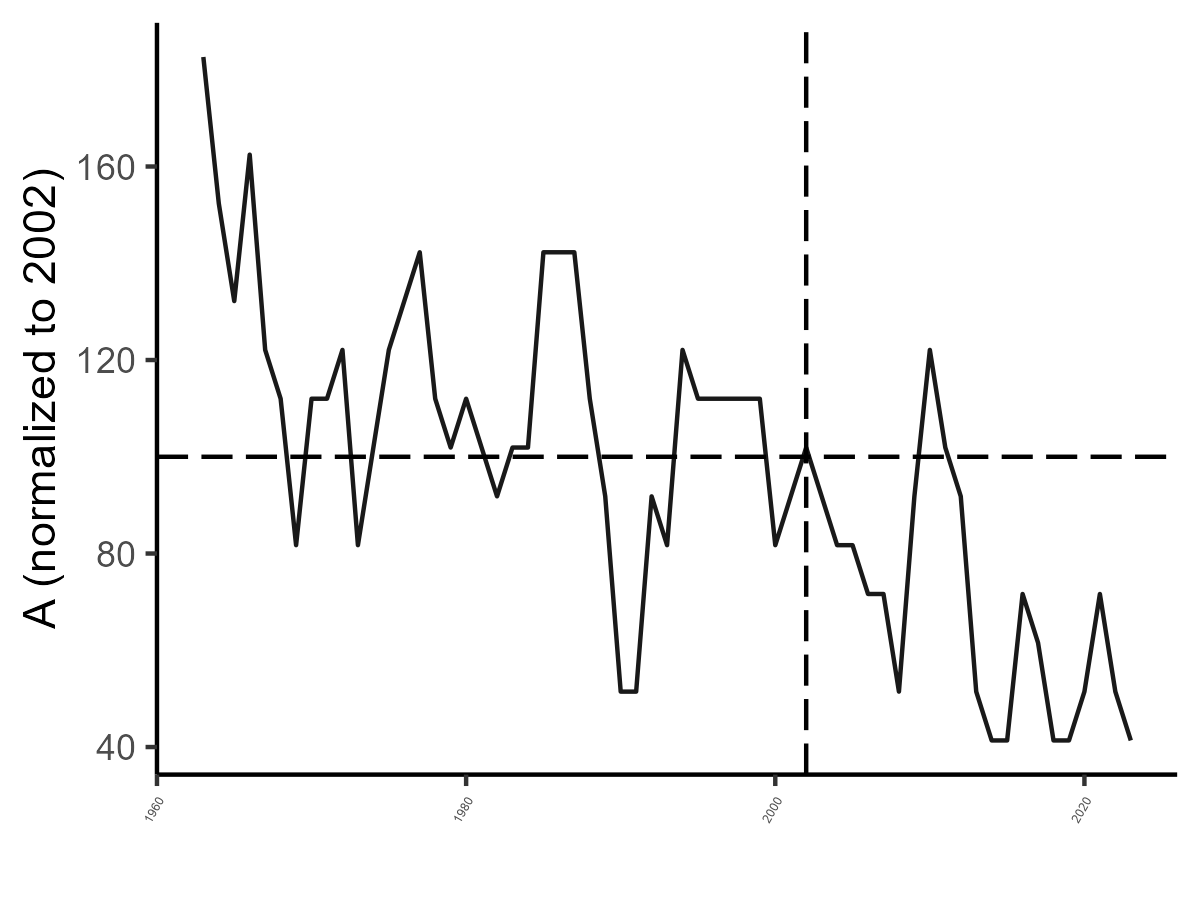
\includegraphics[width = 0.37\textwidth]
  {figuretable/matching_efficiency_year.png}}
  \subfloat[Matching Elasticity ($\frac{d\ln M}{d\ln U}$, $\frac{d\ln M}{d\ln V}$)]{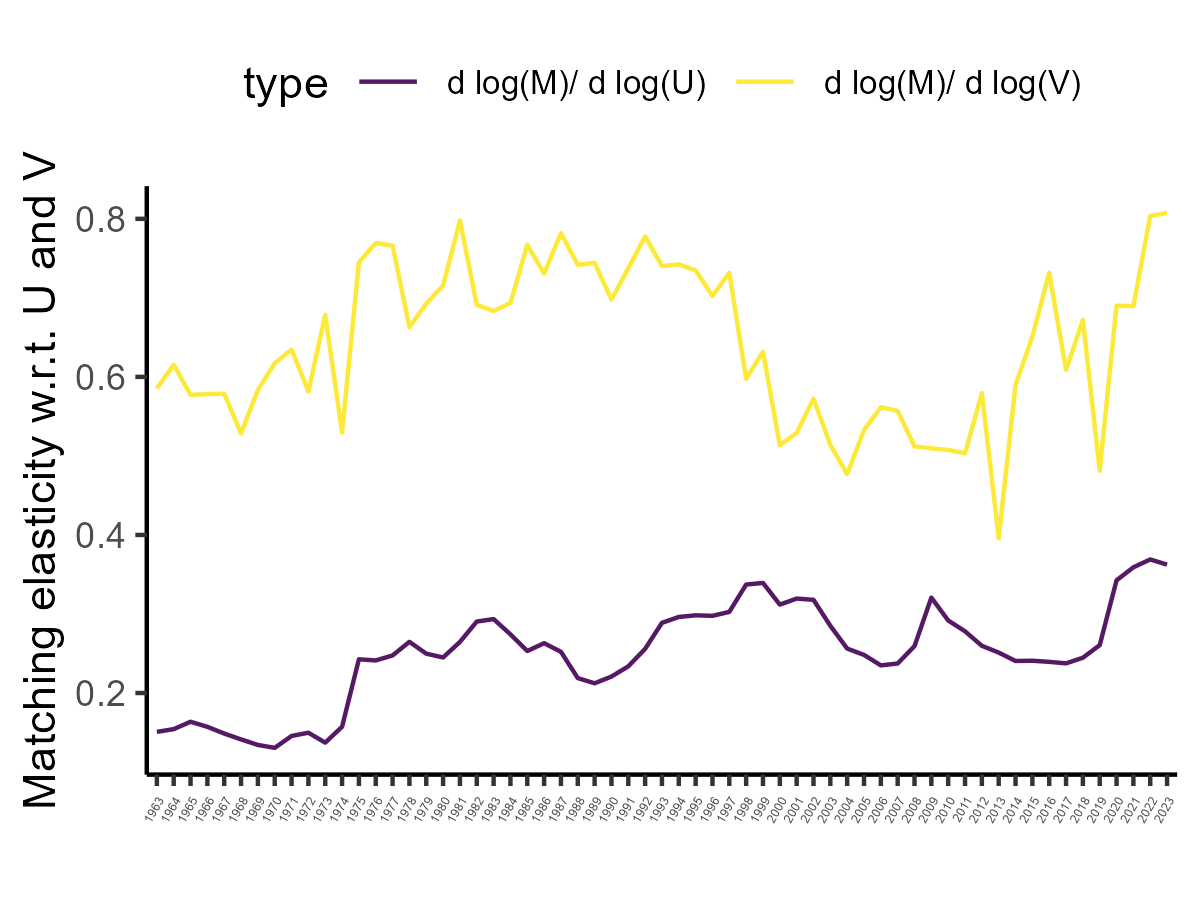
\includegraphics[width = 0.37\textwidth]
  {figuretable/elasticity_year.png}}\\
  \subfloat[Efficiency ($A$) and Tightness ($\ln\frac{V}{U}$)]{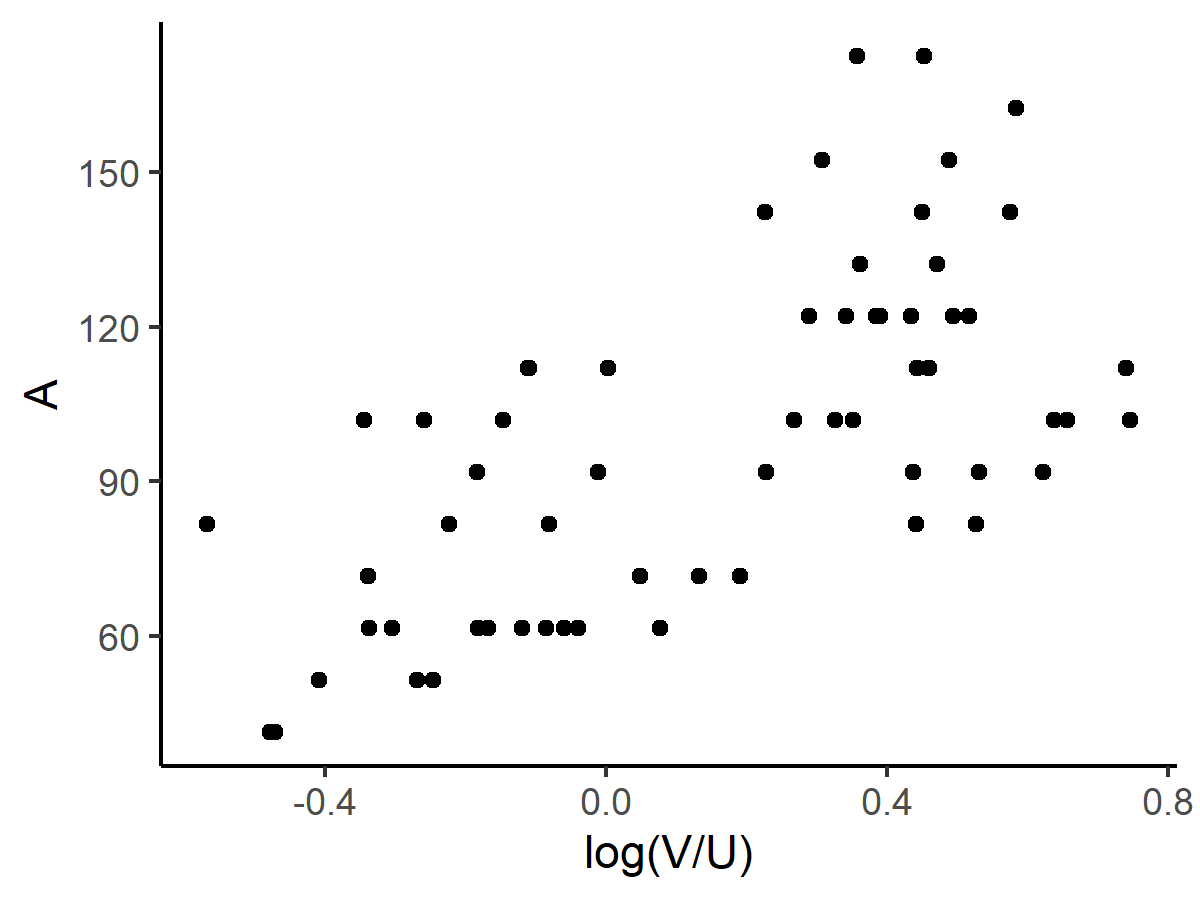
\includegraphics[width = 0.37\textwidth]
  {figuretable/efficiency_tightness_plot_year.png}}
  \subfloat[Efficiency ($A$) and ($\ln \frac{M}{U}$, $\ln \frac{M}{V}$)]{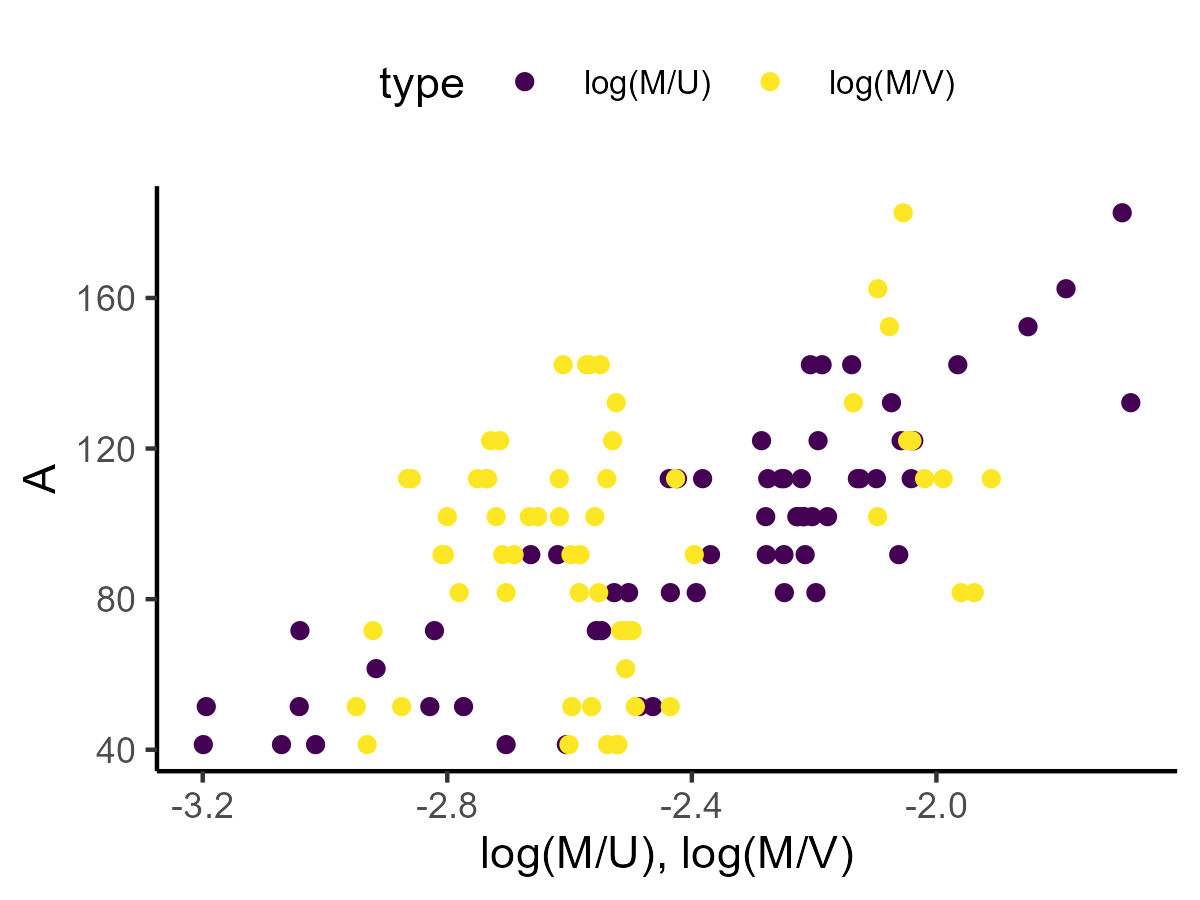
\includegraphics[width = 0.37\textwidth]
  {figuretable/job_finding_rate_efficiency_plot_year.png}}
  \caption{Year-level results 1966-2024}
  \label{fg:year_results} 
  \end{center}
  \footnotesize
  %Note: 
\end{figure} 

Figures \ref{fg:year_results} provide a year-level counterpart to Figure \ref{fg:month_part_and_full_time_results}. Figures \ref{fg:year_results} (a)-(d) provide annual data patterns of unemployed individuals, vacancies, labor market tightness (\(V/U\)), hires, the  ($U$,$V$) relationship, and job and worker finding rates (\(M/U\) and \(M/V\)). In summary, the numbers of unemployed individuals and vacancies increase with fluctuations, corresponding with market tightness, while the number of hires shows a noticeable decline until around the mid-1980s, peaks and troughs from the mid-1980s to the late 1990s, and a sharp decline towards recent years.

Figures \ref{fg:year_results} (e) and (f) present the estimation results of the matching function along with matching efficiency and elasticities (\(\frac{d\ln M}{d\ln U}\) and \(\frac{d\ln M}{d\ln V}\)). Notably, matching efficiency (normalized to 1972) shows a declining trend with notable fluctuations, which is consistent with the downward trends of job and worker finding rates. This might be due to an increase in matching opportunities outside of the government-operated platform.

The implied match elasticity with respect to unemployment is 0.8-1.2, which is higher than previous worldwide findings such as \cite{petrongolo2001looking} (range: 0.5-0.7) and Japanese studies such as \cite{higashi2018spatial} (0.38 for 2000-2014 monthly), \cite{kawata2019} (0.48 for 2012-2017 prefecture-month-level), \cite{kano2005estimating} (0.56 for 1972-1999 prefecture-year-level), \cite{sasaki2007measuring} (about 0.6 for 1998-2007 prefecture-quarter-level), and \cite{kambayashi2006vacancy} (about 0.8 for 1996-2001 prefecture-month-level). 

On the other hand, the implied match elasticity with respect to vacancies is 0.1-0.3, which is comparable to \cite{lange2020beyond} (range: 0.3-0.5) and Japanese studies such as \cite{higashi2018spatial} (0.24 for 2000-2014 monthly), \cite{kawata2019} (0.52 for 2012-2017 prefecture-month-level), \cite{kano2005estimating} (0.3 for 1972-1999 prefecture-year-level), \cite{sasaki2007measuring} (about 0.2 for 1998-2007 prefecture-quarter-level), and \cite{kambayashi2006vacancy} (about 0.3 for 1996-2001 prefecture-month-level).

Figures \ref{fg:year_results} (g) and (h) illustrate some correlation patterns between matching efficiency and market structure variables such as labor market tightness, worker finding rate, and job finding rate. Consistent with \cite{lange2020beyond}, these highlight positive correlations between efficiency and market structure, such as tightness, which induce a positive bias in the estimates of the vacancy elasticity whenever unobserved matching efficacy is not controlled for, as is the case in traditional estimators.


\textcolor{blue}{Note that I normalize the location of matching efficiency in January 2002 to 100 for comparison with Figure \ref{fg:month_part_and_full_time_results}, which is normalized to 2002.
Also, note that the monthly data is not a complete subset of the annual data, so both estimates differ. 
The monthly data patterns are almost consistent with the year-level ones, except for seasonal fluctuations. The only remarkable difference from the year-level results is that the implied match elasticity with respect to vacancies is 0.6-1.2, relative to 0.1-0.3 at the month level. This discrepancy arises because the estimated coefficient and the scale of matching efficiency differ across datasets. 
For example, the monthly matching efficiency around 2010 is 210, whereas the yearly one is 120 because the observed maximum of each efficiency is in 1966 for yearly analysis and exists in 2010 for monthly analysis.
Although \cite{lange2020beyond} do not explicitly mention the issue of scale normalization, this highlights the difficulty of comparing the level of matching efficiency across different datasets. Therefore, we can only compare the efficiency trends.}

\end{document}









